\documentclass[]{article}
\usepackage{lmodern}
\usepackage{amssymb,amsmath}
\usepackage{ifxetex,ifluatex}
\usepackage{fixltx2e} % provides \textsubscript
\ifnum 0\ifxetex 1\fi\ifluatex 1\fi=0 % if pdftex
  \usepackage[T1]{fontenc}
  \usepackage[utf8]{inputenc}
\else % if luatex or xelatex
  \ifxetex
    \usepackage{mathspec}
  \else
    \usepackage{fontspec}
  \fi
  \defaultfontfeatures{Ligatures=TeX,Scale=MatchLowercase}
\fi
% use upquote if available, for straight quotes in verbatim environments
\IfFileExists{upquote.sty}{\usepackage{upquote}}{}
% use microtype if available
\IfFileExists{microtype.sty}{%
\usepackage{microtype}
\UseMicrotypeSet[protrusion]{basicmath} % disable protrusion for tt fonts
}{}
\usepackage[margin=1in]{geometry}
\usepackage{hyperref}
\hypersetup{unicode=true,
            pdftitle={MAthesis},
            pdfborder={0 0 0},
            breaklinks=true}
\urlstyle{same}  % don't use monospace font for urls
\usepackage{natbib}
\bibliographystyle{plainnat}
\usepackage{longtable,booktabs}
\usepackage{graphicx,grffile}
\makeatletter
\def\maxwidth{\ifdim\Gin@nat@width>\linewidth\linewidth\else\Gin@nat@width\fi}
\def\maxheight{\ifdim\Gin@nat@height>\textheight\textheight\else\Gin@nat@height\fi}
\makeatother
% Scale images if necessary, so that they will not overflow the page
% margins by default, and it is still possible to overwrite the defaults
% using explicit options in \includegraphics[width, height, ...]{}
\setkeys{Gin}{width=\maxwidth,height=\maxheight,keepaspectratio}
\IfFileExists{parskip.sty}{%
\usepackage{parskip}
}{% else
\setlength{\parindent}{0pt}
\setlength{\parskip}{6pt plus 2pt minus 1pt}
}
\setlength{\emergencystretch}{3em}  % prevent overfull lines
\providecommand{\tightlist}{%
  \setlength{\itemsep}{0pt}\setlength{\parskip}{0pt}}
\setcounter{secnumdepth}{0}
% Redefines (sub)paragraphs to behave more like sections
\ifx\paragraph\undefined\else
\let\oldparagraph\paragraph
\renewcommand{\paragraph}[1]{\oldparagraph{#1}\mbox{}}
\fi
\ifx\subparagraph\undefined\else
\let\oldsubparagraph\subparagraph
\renewcommand{\subparagraph}[1]{\oldsubparagraph{#1}\mbox{}}
\fi

%%% Use protect on footnotes to avoid problems with footnotes in titles
\let\rmarkdownfootnote\footnote%
\def\footnote{\protect\rmarkdownfootnote}

%%% Change title format to be more compact
\usepackage{titling}

% Create subtitle command for use in maketitle
\newcommand{\subtitle}[1]{
  \posttitle{
    \begin{center}\large#1\end{center}
    }
}

\setlength{\droptitle}{-2em}
  \title{MAthesis}
  \pretitle{\vspace{\droptitle}\centering\huge}
  \posttitle{\par}
  \author{}
  \preauthor{}\postauthor{}
  \date{}
  \predate{}\postdate{}

\usepackage{setspace}
\doublespacing

\begin{document}
\maketitle

{
\setcounter{tocdepth}{2}
\tableofcontents
}
\section{Time Bins with sample sizes}\label{time-bins-with-sample-sizes}

\begin{longtable}[]{@{}llrrrr@{}}
\caption{Time bins with age range, epoch name, mean age and
corresponding sample sizes (on individual, species and genus
level)}\tabularnewline
\toprule
bin & EpochBins & MeanBins & nIndividuals & nSpecies &
nGenera\tabularnewline
\midrule
\endfirsthead
\toprule
bin & EpochBins & MeanBins & nIndividuals & nSpecies &
nGenera\tabularnewline
\midrule
\endhead
(0,0.0117{]} & Modern & 0.00585 & 252 & 64 & 18\tabularnewline
(0.0117,0.126{]} & Upper Pleistocene & 0.06885 & 47 & 16 &
8\tabularnewline
(0.126,0.781{]} & Middle Pleistocene & 0.45350 & 48 & 11 &
6\tabularnewline
(0.781,2.59{]} & Lower Pleistocene & 1.68450 & 73 & 27 &
11\tabularnewline
(2.59,3.6{]} & Upper Pliocene & 3.09400 & 23 & 15 & 9\tabularnewline
(3.6,5.33{]} & Lower Pliocene & 4.46600 & 29 & 17 & 8\tabularnewline
(5.33,11.6{]} & Upper Miocene & 8.47000 & 52 & 23 & 9\tabularnewline
(11.6,16{]} & Middle Miocene & 13.78900 & 38 & 17 & 11\tabularnewline
(16,23{]} & Lower Miocene & 19.50000 & 25 & 13 & 9\tabularnewline
(23,50{]} & Oligocene and Eocene & 36.51500 & 7 & 5 & 5\tabularnewline
\bottomrule
\end{longtable}

\section{Maps}\label{maps}

\subsection{fossil occurences of
testudinidae}\label{fossil-occurences-of-testudinidae}

\begin{figure}[htbp]
\centering
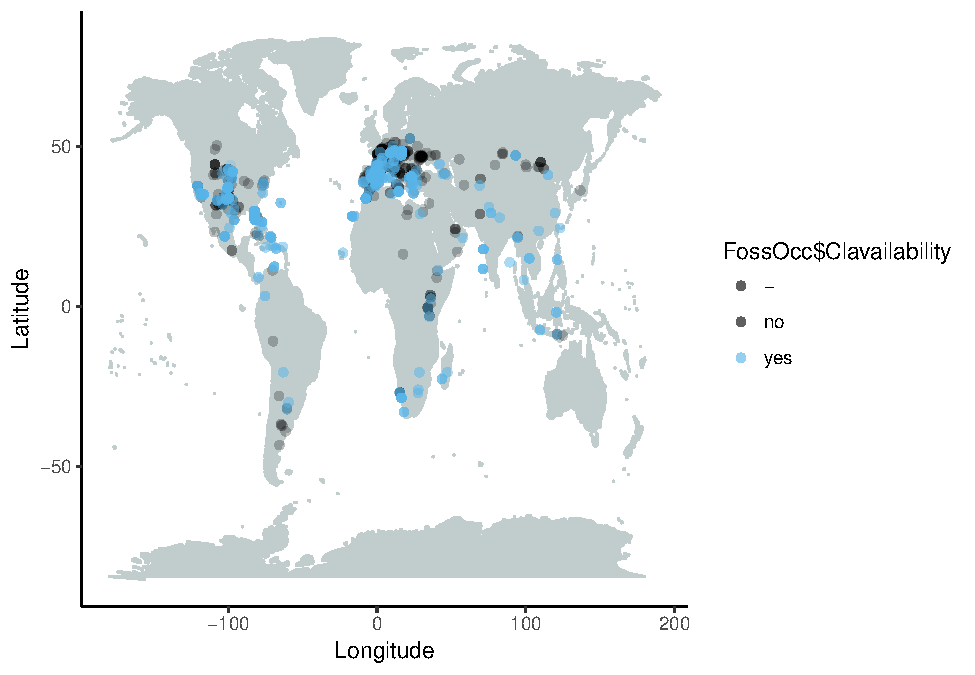
\includegraphics{MA_JJ_files/figure-latex/Map fossil occurrences-1.pdf}
\caption{Map displaying all fossil occurrences of testudinids, with
color indicating whether relevant literature was available (black if
not) and if it was, whether body size data was available or not (yes and
no, respectively).}
\end{figure}

\subsection{body size of testudinidae}\label{body-size-of-testudinidae}

\begin{figure}[htbp]
\centering
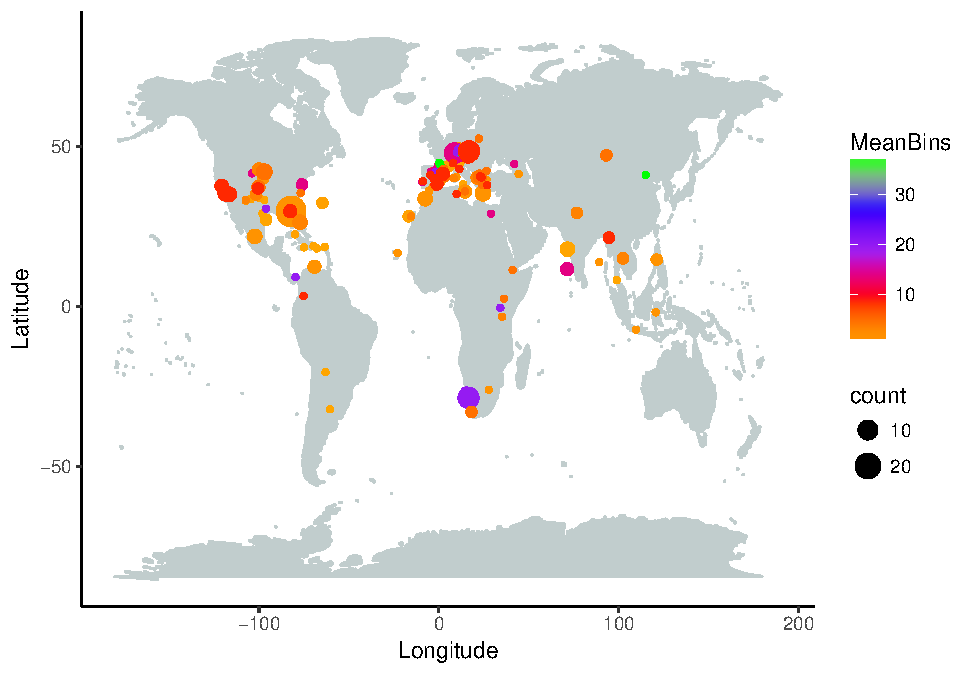
\includegraphics{MA_JJ_files/figure-latex/Map body size data set-1.pdf}
\caption{Map displaying all localities for which body size data for
testudinids was available in the literature. Size of points denotes
sample size, color denotes approximate age.}
\end{figure}

\section{Sampling Accumulation Curve}\label{sampling-accumulation-curve}

\begin{figure}[htbp]
\centering
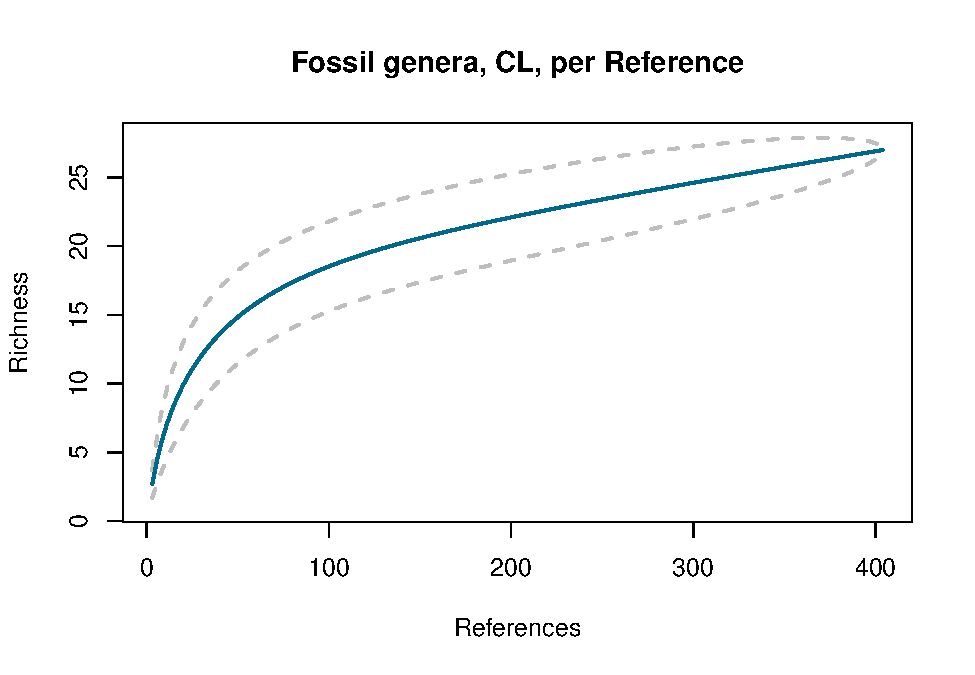
\includegraphics{MA_JJ_files/figure-latex/Species Accumulation Curve with Genera-1.pdf}
\caption{Sampling Accumulation Curve of fossil genera per reference}
\end{figure}

\newpage

\section{Histograms}\label{histograms}

\subsection{all}\label{all}

\begin{verbatim}
## `stat_bin()` using `bins = 30`. Pick better value with `binwidth`.
\end{verbatim}

\begin{figure}[htbp]
\centering
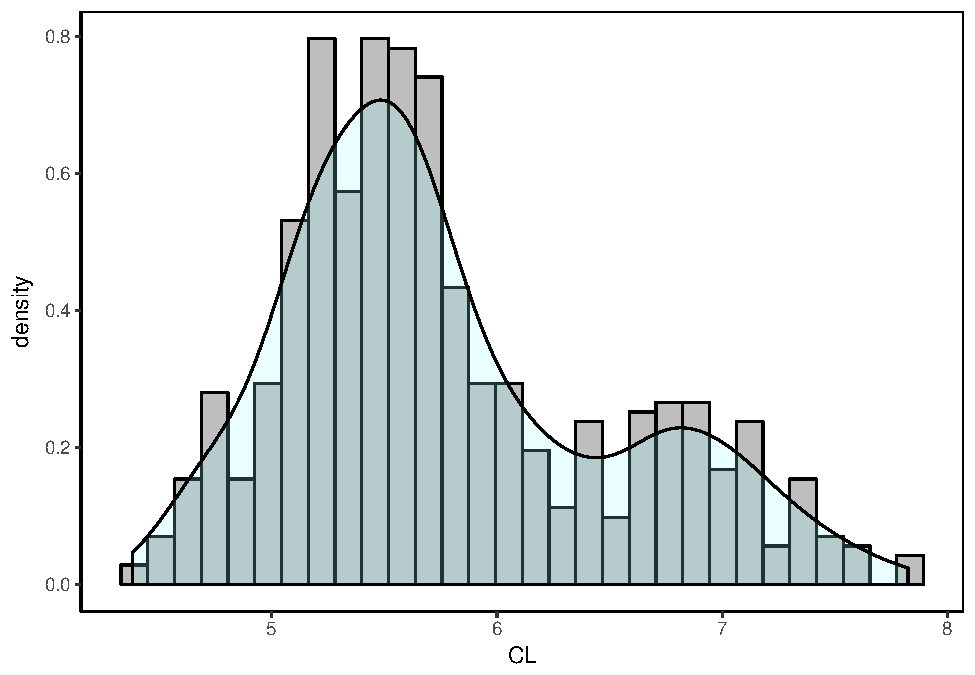
\includegraphics{MA_JJ_files/figure-latex/Histograms of body size data, all-1.pdf}
\caption{Distribution of body size data, logtransformed, all data.}
\end{figure}

\subsection{per time bin}\label{per-time-bin}

\begin{verbatim}
## `stat_bin()` using `bins = 30`. Pick better value with `binwidth`.
\end{verbatim}

\begin{figure}[htbp]
\centering
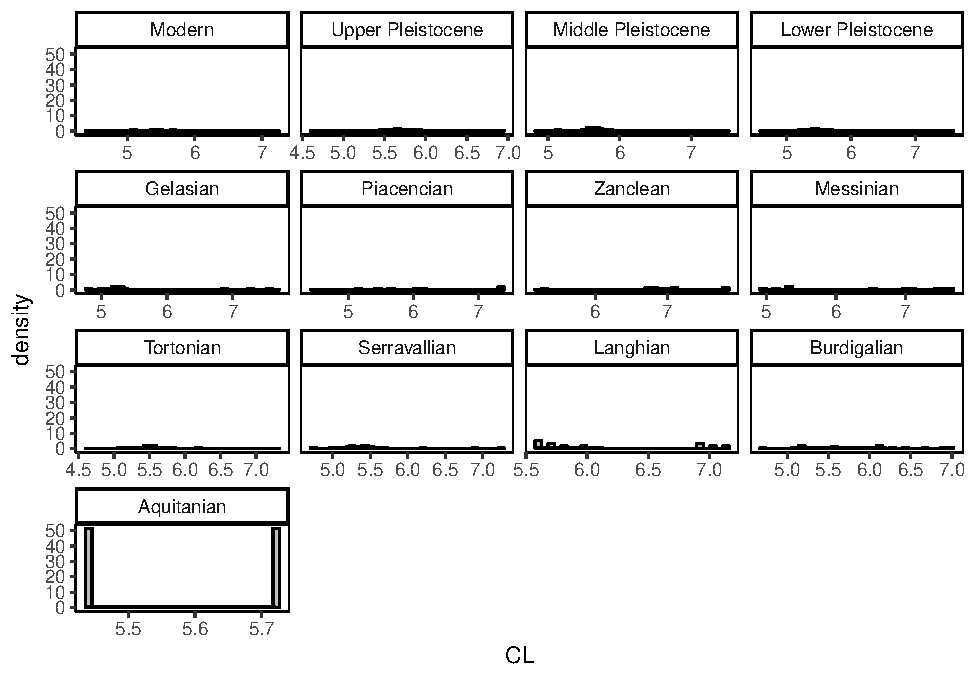
\includegraphics{MA_JJ_files/figure-latex/Histograms of body size data, per time bin-1.pdf}
\caption{Distribution of body size data per time bin, logtransformed.}
\end{figure}

\subsection{continental vs.~insular}\label{continental-vs.insular}

\begin{verbatim}
## `stat_bin()` using `bins = 30`. Pick better value with `binwidth`.
\end{verbatim}

\begin{figure}[htbp]
\centering
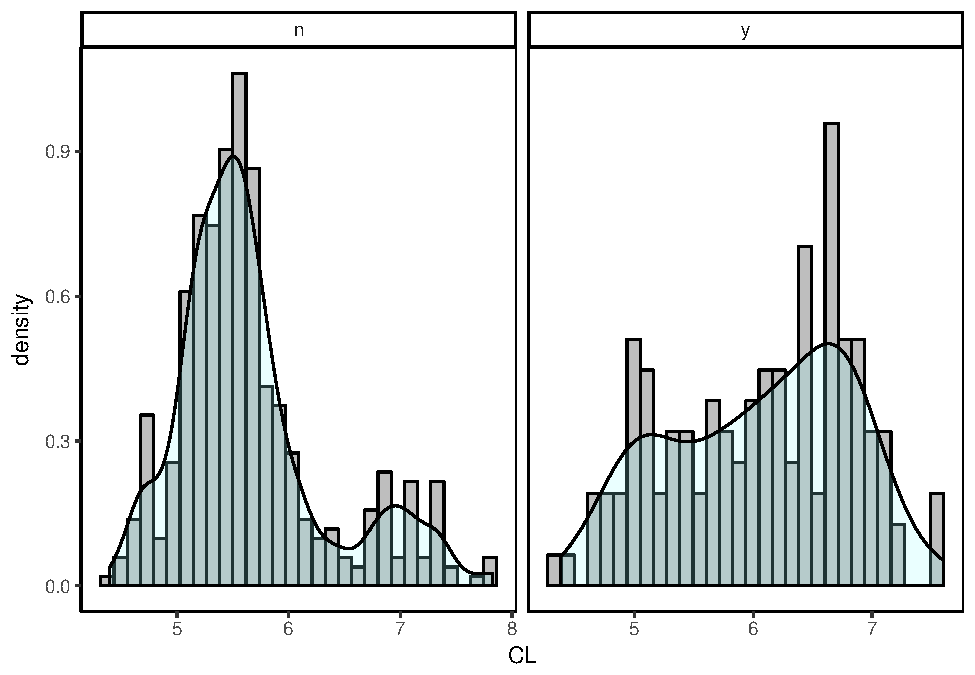
\includegraphics{MA_JJ_files/figure-latex/Histograms of body size data, continental vs. insular-1.pdf}
\caption{Distribution of body site data of continental (n) and
insular(y) species, logtransformed.}
\end{figure}

\subsection{continents}\label{continents}

\begin{verbatim}
## `stat_bin()` using `bins = 30`. Pick better value with `binwidth`.
\end{verbatim}

\begin{figure}[htbp]
\centering
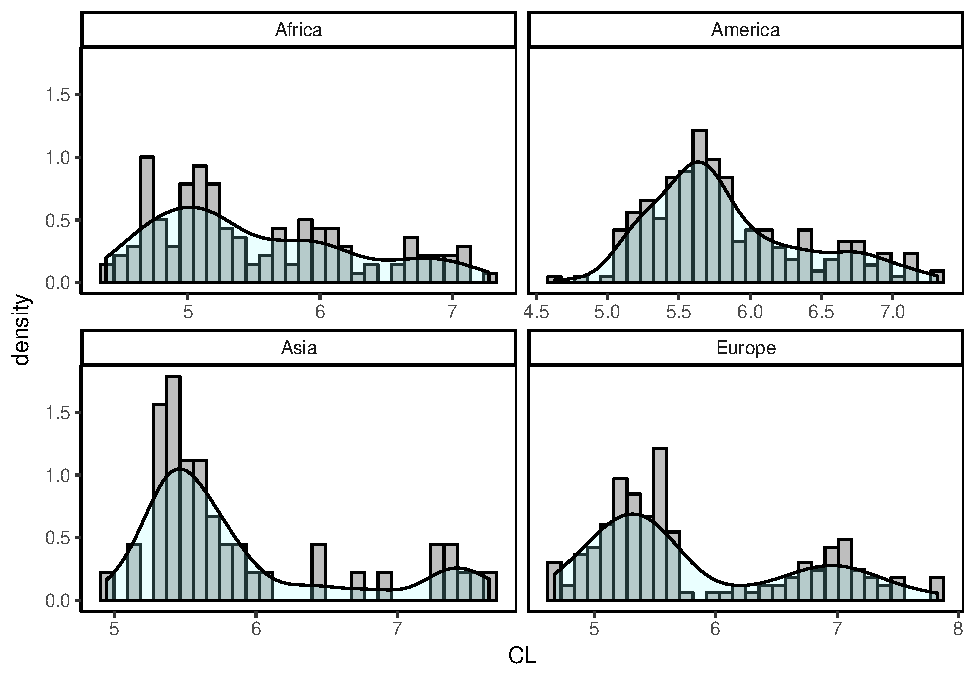
\includegraphics{MA_JJ_files/figure-latex/Histograms of body size data, split by continents-1.pdf}
\caption{Distribution of body site data of continental (n) and
insular(y) species, logtransformed.}
\end{figure}

\newpage

\begin{longtable}[]{@{}rrrrrrrrrrrrl@{}}
\caption{General statistics of body size data: all, per time bin,
insular and continental}\tabularnewline
\toprule
nCL & min & max & var & mean & logm & med & logmed & skew & logsk & kurt
& logku & Variable\tabularnewline
\midrule
\endfirsthead
\toprule
nCL & min & max & var & mean & logm & med & logmed & skew & logsk & kurt
& logku & Variable\tabularnewline
\midrule
\endhead
573 & 80.00 & 2500 & 146793.95 & 419.2 & 2.5 & 270.0 & 2.4 & 2.30 & 0.70
& 9.25 & 2.84 & all\tabularnewline
251 & 80.00 & 1300 & 67716.64 & 328.9 & 2.4 & 242.0 & 2.4 & 1.85 & 0.60
& 5.91 & 2.73 & Modern\tabularnewline
46 & 102.44 & 1250 & 69637.75 & 438.4 & 2.6 & 331.1 & 2.5 & 1.30 & 0.29
& 3.89 & 2.69 & Upper Pleistocene\tabularnewline
47 & 132.00 & 1500 & 64523.61 & 357.3 & 2.5 & 285.6 & 2.5 & 2.99 & 1.58
& 12.00 & 5.93 & Middle Pleistocene\tabularnewline
71 & 107.80 & 2000 & 176257.96 & 417.4 & 2.5 & 224.1 & 2.4 & 2.08 & 1.06
& 6.77 & 2.99 & Lower Pleistocene\tabularnewline
20 & 165.00 & 1600 & 269797.71 & 636.6 & 2.7 & 440.5 & 2.6 & 0.96 & 0.29
& 2.38 & 1.78 & Upper Pliocene\tabularnewline
24 & 176.00 & 2500 & 516172.48 & 953.5 & 2.8 & 847.5 & 2.9 & 1.08 &
-0.31 & 3.32 & 2.13 & Lower Pliocene\tabularnewline
49 & 107.00 & 2100 & 274774.35 & 542.8 & 2.6 & 250.0 & 2.4 & 1.46 & 0.66
& 4.00 & 2.17 & Upper Miocene\tabularnewline
34 & 111.00 & 1500 & 169511.65 & 454.8 & 2.5 & 255.0 & 2.4 & 1.32 & 0.83
& 3.16 & 2.29 & Middle Miocene\tabularnewline
24 & 160.00 & 1100 & 81679.97 & 425.8 & 2.5 & 317.0 & 2.5 & 1.20 & 0.48
& 3.25 & 2.06 & Lower Miocene\tabularnewline
7 & 275.00 & 635 & 15613.99 & 453.2 & 2.6 & 412.5 & 2.6 & 0.29 & -0.17 &
2.06 & 2.36 & Oligocene and Eocene\tabularnewline
434 & 81.00 & 2500 & 137816.81 & 375.5 & 2.5 & 250.0 & 2.4 & 2.90 & 1.08
& 12.62 & 3.97 & continental\tabularnewline
139 & 80.00 & 2000 & 151260.27 & 555.7 & 2.6 & 466.0 & 2.7 & 1.08 &
-0.24 & 4.33 & 2.01 & insular\tabularnewline
140 & 80.00 & 1446 & 92601.87 & 337.4 & 2.4 & 193.5 & 2.3 & 1.69 & 0.64
& 5.04 & 2.35 & Africa\tabularnewline
230 & 102.44 & 1500 & 73060.64 & 402.7 & 2.5 & 300.0 & 2.5 & 1.85 & 0.77
& 6.10 & 2.97 & America\tabularnewline
49 & 140.00 & 2100 & 286030.39 & 505.9 & 2.6 & 275.0 & 2.4 & 1.87 & 1.28
& 5.03 & 3.29 & Asia\tabularnewline
154 & 107.00 & 2500 & 251479.46 & 490.8 & 2.5 & 245.0 & 2.4 & 1.95 &
0.77 & 6.86 & 2.32 & Europe\tabularnewline
\bottomrule
\end{longtable}

\section{Boxplots}\label{boxplots}

\subsection{genera per time bins}\label{genera-per-time-bins}

\begin{figure}[htbp]
\centering
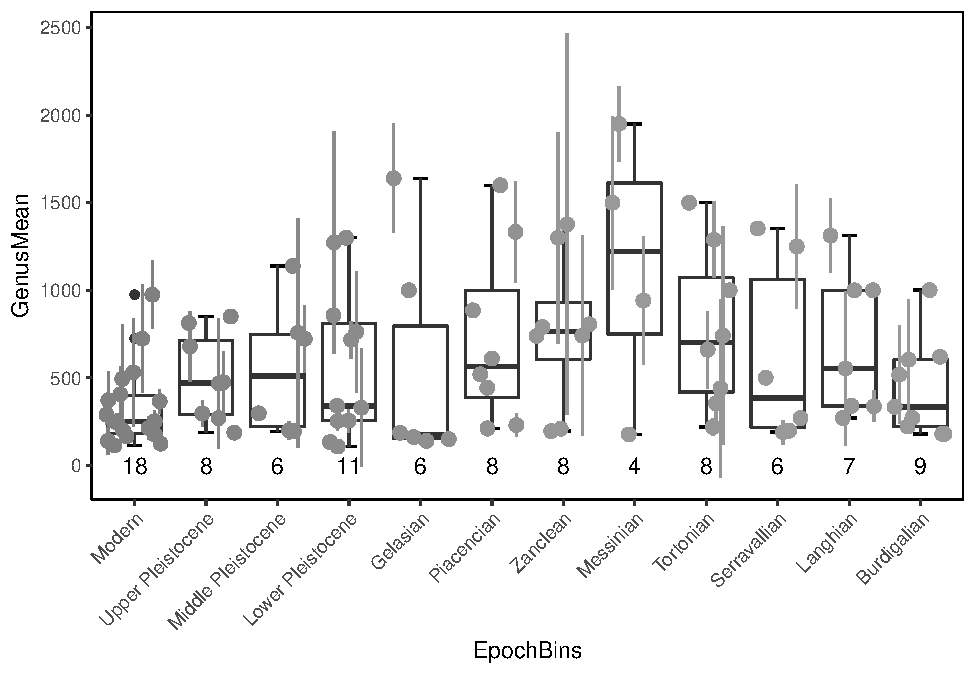
\includegraphics{MA_JJ_files/figure-latex/Boxplots of each genus per time bin-1.pdf}
\caption{Boxplots of mean CL per time bin, including mean and sd CL for
each genus (as pointrange).}
\end{figure}

\subsection{continental vs.~insular per time
bin}\label{continental-vs.insular-per-time-bin}

\begin{figure}[htbp]
\centering
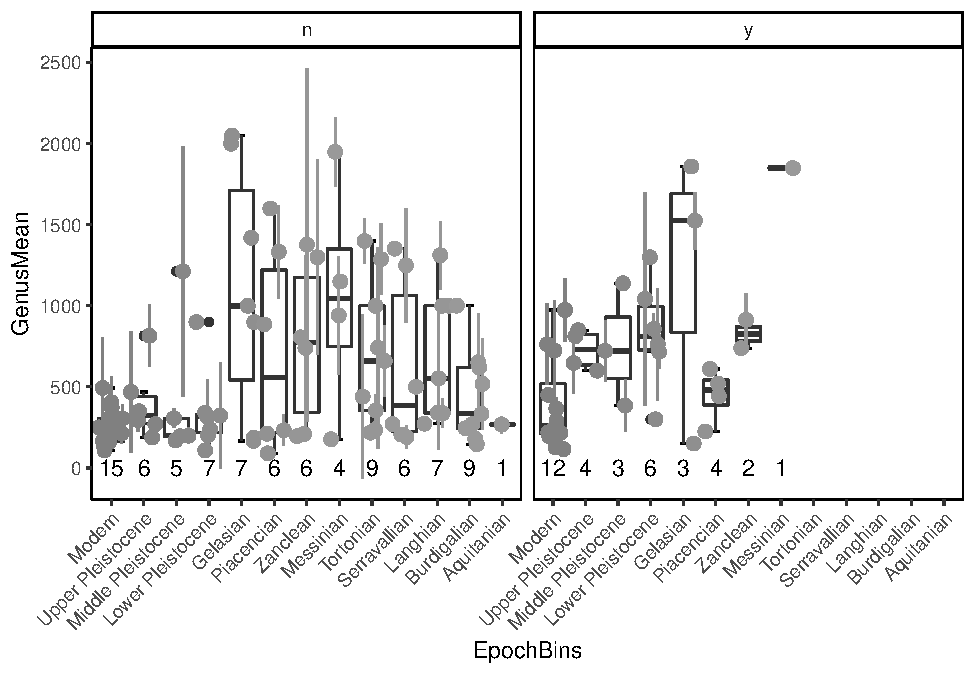
\includegraphics{MA_JJ_files/figure-latex/Boxplots of each genus per time bin, continental vs. insular-1.pdf}
\caption{Boxplots of each genus per time bin, continental vs.~insular
species.}
\end{figure}

\subsection{continental vs.~insular}\label{continental-vs.insular-1}

\begin{verbatim}
## Warning: Removed 9 rows containing missing values (geom_pointrange).
\end{verbatim}

\begin{figure}[htbp]
\centering
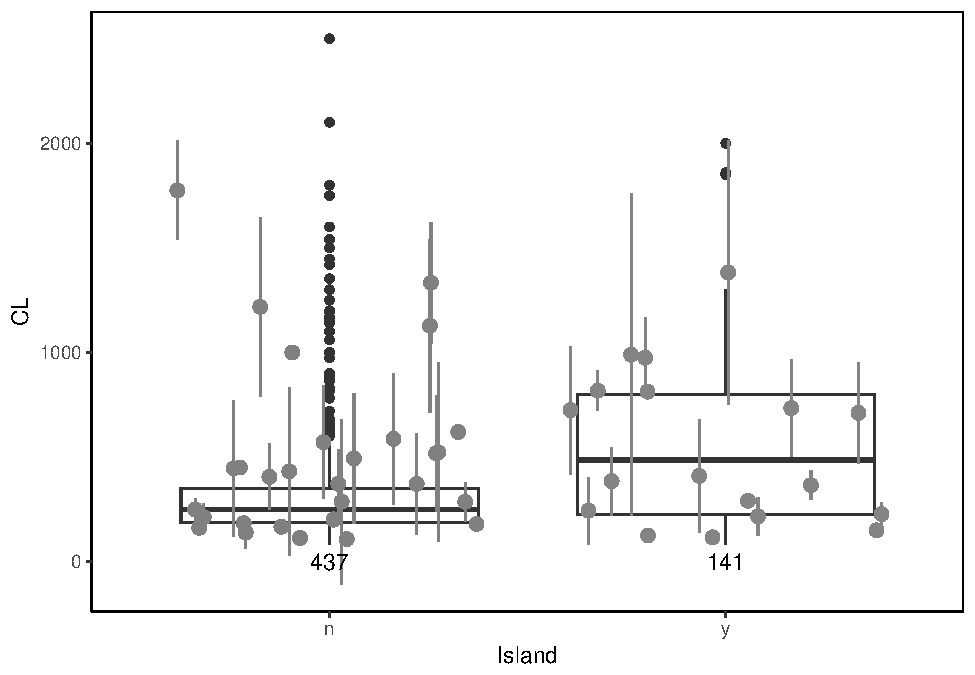
\includegraphics{MA_JJ_files/figure-latex/Boxplot continental vs. insular-1.pdf}
\caption{Boxplot continental vs.~insular, genera summarised}
\end{figure}

\subsection{continental vs.~insular per time
bin}\label{continental-vs.insular-per-time-bin-1}

\begin{figure}[htbp]
\centering
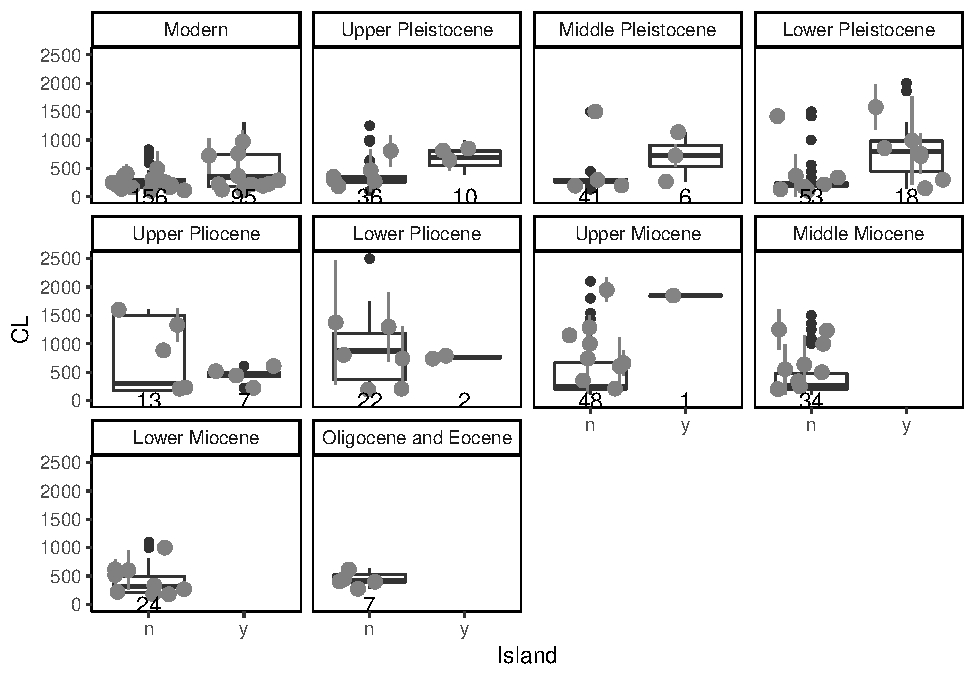
\includegraphics{MA_JJ_files/figure-latex/Boxplot continental vs. insular, split into time bins-1.pdf}
\caption{Boxplot continental vs.~insular, genera summarised}
\end{figure}

\subsection{continents}\label{continents-1}

\begin{figure}[htbp]
\centering
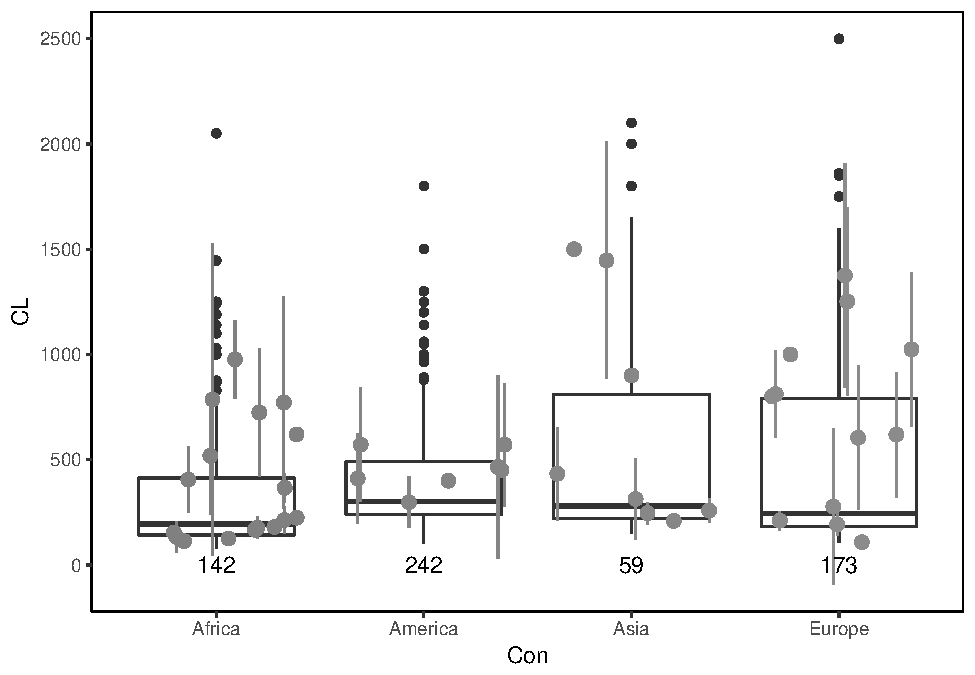
\includegraphics{MA_JJ_files/figure-latex/Boxplot body size split into continents-1.pdf}
\caption{Boxplot: body size on different continents, genera summarised}
\end{figure}

\newpage

\section{paleoTS analysis}\label{paleots-analysis}

\subsection{all (continental and
insular)}\label{all-continental-and-insular}

\subsubsection{individuals (all)}\label{individuals-all}

\begin{figure}[htbp]
\centering
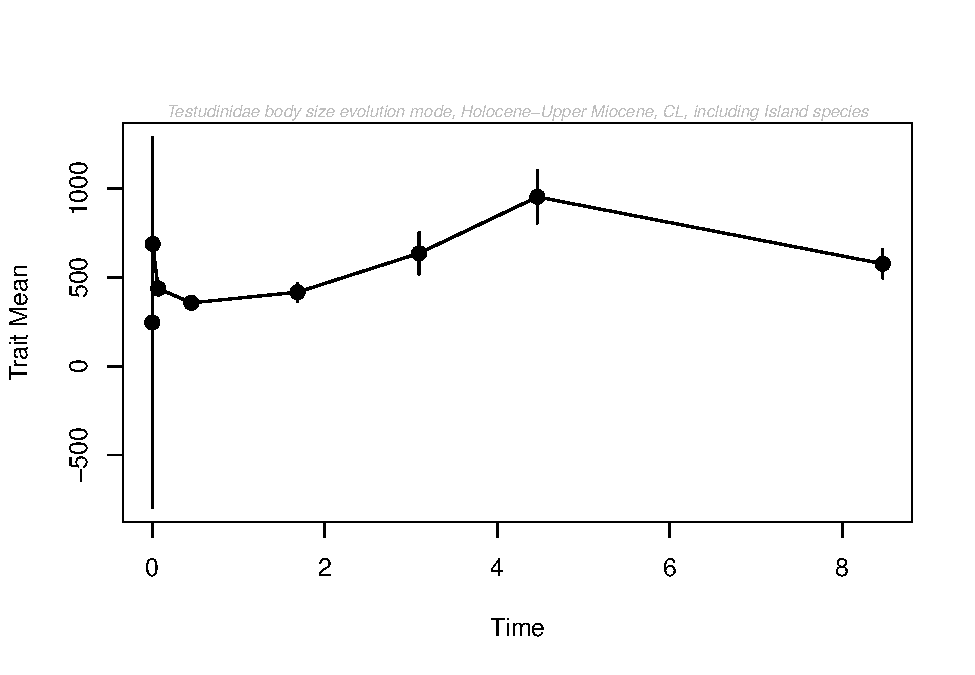
\includegraphics{MA_JJ_files/figure-latex/paleoTS plot-1.pdf}
\caption{individuals, including island species}
\end{figure}

\begin{longtable}[]{@{}lrrrr@{}}
\caption{Model-fitting results for testudinidae, individuals, including
island species}\tabularnewline
\toprule
& logL & K & AICc & Akaike.wt\tabularnewline
\midrule
\endfirsthead
\toprule
& logL & K & AICc & Akaike.wt\tabularnewline
\midrule
\endhead
GRW & -68.07841 & 2 & 141.8711 & 0.008\tabularnewline
URW & -68.07845 & 1 & 138.6569 & 0.040\tabularnewline
Stasis & -63.29025 & 2 & 132.2948 & 0.952\tabularnewline
\bottomrule
\end{longtable}

\newpage

\subsubsection{species (all)}\label{species-all}

\begin{figure}[htbp]
\centering
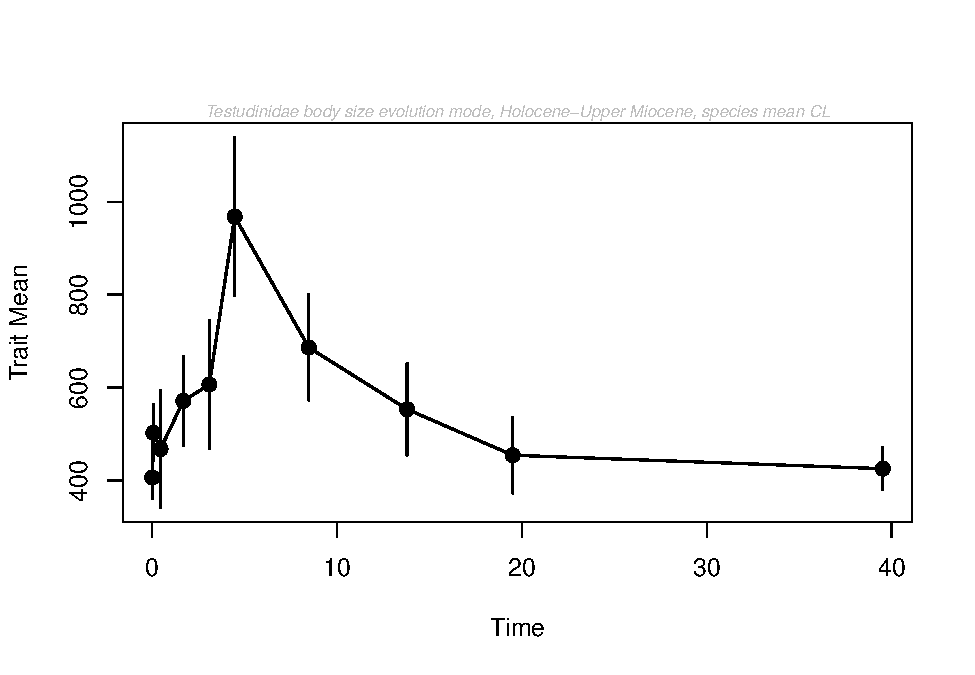
\includegraphics{MA_JJ_files/figure-latex/paleoTS plot with species mean, including island species-1.pdf}
\caption{paleoTS plot with species mean, including island species}
\end{figure}

\begin{longtable}[]{@{}lrrrr@{}}
\caption{Model-fitting results for testudinidae, species, including
island species}\tabularnewline
\toprule
& logL & K & AICc & Akaike.wt\tabularnewline
\midrule
\endfirsthead
\toprule
& logL & K & AICc & Akaike.wt\tabularnewline
\midrule
\endhead
GRW & -56.70310 & 2 & 119.4062 & 0.149\tabularnewline
URW & -56.93847 & 1 & 116.4484 & 0.653\tabularnewline
Stasis & -56.41523 & 2 & 118.8305 & 0.198\tabularnewline
\bottomrule
\end{longtable}

\newpage

\subsubsection{genera (all)}\label{genera-all}

\begin{figure}[htbp]
\centering
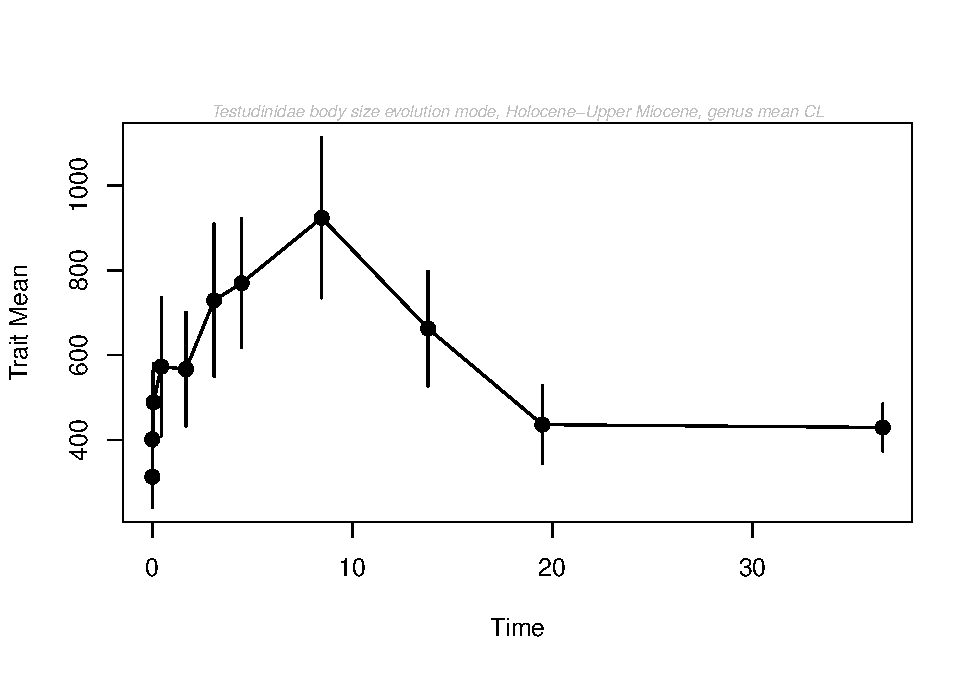
\includegraphics{MA_JJ_files/figure-latex/paleoTS plot with genus mean, including island species-1.pdf}
\caption{paleoTS plot with genus mean, including island species}
\end{figure}

\begin{longtable}[]{@{}lrrrr@{}}
\caption{Model-fitting results for testudinidae, genera, including
island species}\tabularnewline
\toprule
& logL & K & AICc & Akaike.wt\tabularnewline
\midrule
\endfirsthead
\toprule
& logL & K & AICc & Akaike.wt\tabularnewline
\midrule
\endhead
GRW & -64.78186 & 2 & 135.2780 & 0.166\tabularnewline
URW & -64.86224 & 1 & 132.2245 & 0.766\tabularnewline
Stasis & -65.68705 & 2 & 137.0884 & 0.067\tabularnewline
\bottomrule
\end{longtable}

\newpage

\subsection{continental (excluding insular
species)}\label{continental-excluding-insular-species}

\subsubsection{individuals (continental)}\label{individuals-continental}

\begin{figure}[htbp]
\centering
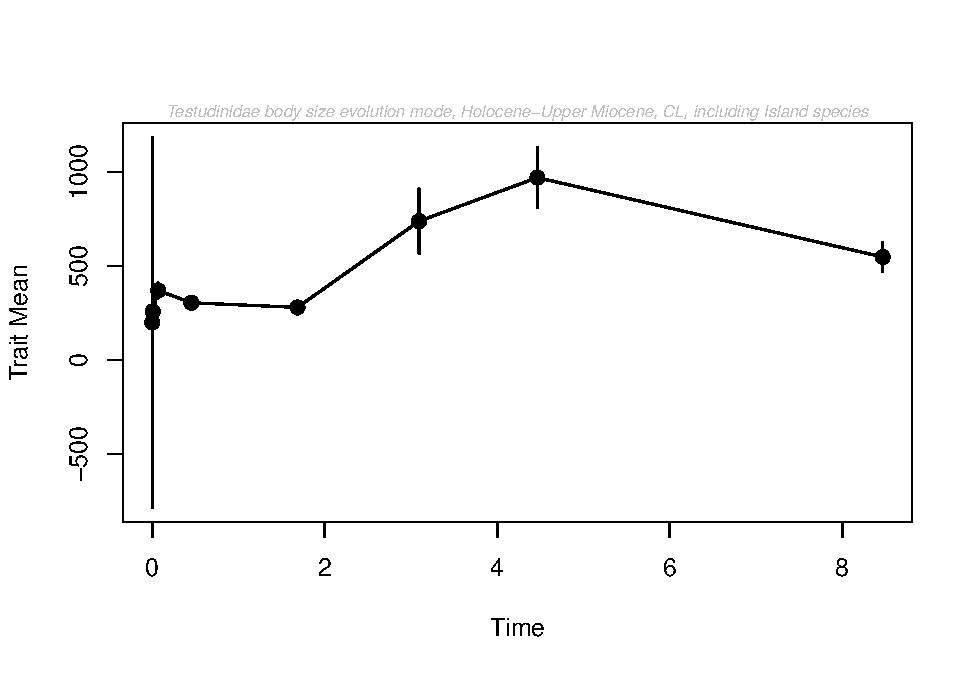
\includegraphics{MA_JJ_files/figure-latex/paleoTS, individuals, exluding island species-1.pdf}
\caption{individuals, excluding island species}
\end{figure}

\begin{longtable}[]{@{}lrrrr@{}}
\caption{Model-fitting results for testudinidae, individuals, excluding
island species}\tabularnewline
\toprule
& logL & K & AICc & Akaike.wt\tabularnewline
\midrule
\endfirsthead
\toprule
& logL & K & AICc & Akaike.wt\tabularnewline
\midrule
\endhead
GRW & -70.13728 & 2 & 145.9888 & 0.018\tabularnewline
URW & -70.14070 & 1 & 142.7814 & 0.090\tabularnewline
Stasis & -66.24073 & 2 & 138.1957 & 0.892\tabularnewline
\bottomrule
\end{longtable}

\newpage

\subsubsection{species (continental)}\label{species-continental}

\begin{figure}[htbp]
\centering
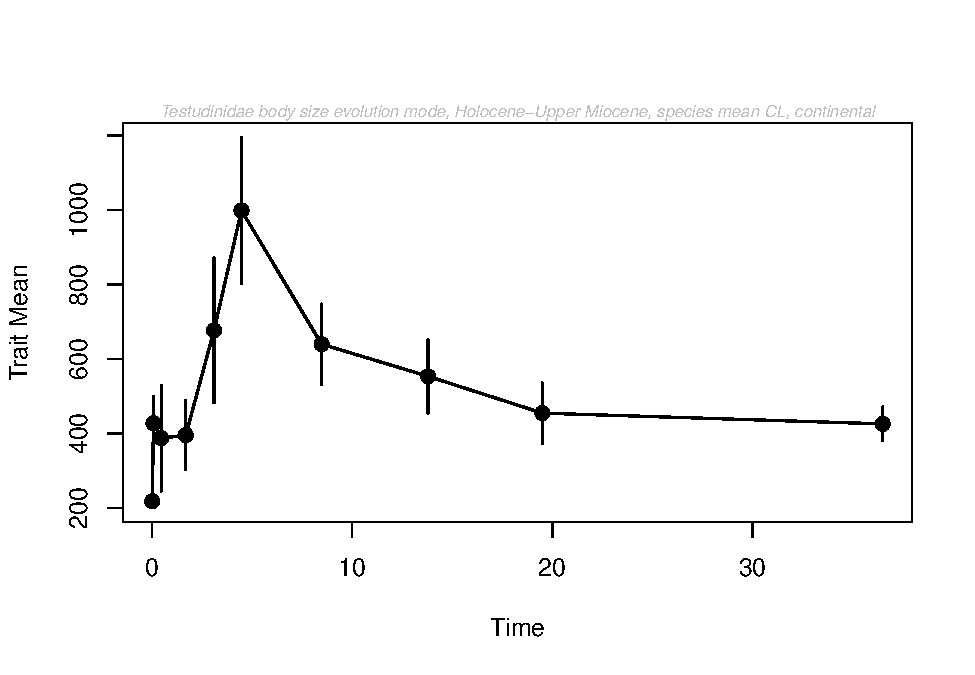
\includegraphics{MA_JJ_files/figure-latex/paleoTS plot with species mean, excluding island species-1.pdf}
\caption{paleoTS plot with species mean, excluding island species}
\end{figure}

\begin{longtable}[]{@{}lrrrr@{}}
\caption{Model-fitting results for testudinidae, species, excluding
island species}\tabularnewline
\toprule
& logL & K & AICc & Akaike.wt\tabularnewline
\midrule
\endfirsthead
\toprule
& logL & K & AICc & Akaike.wt\tabularnewline
\midrule
\endhead
GRW & -60.91398 & 2 & 127.8280 & 0.020\tabularnewline
URW & -62.36871 & 1 & 127.3088 & 0.026\tabularnewline
Stasis & -57.04727 & 2 & 120.0945 & 0.954\tabularnewline
\bottomrule
\end{longtable}

\newpage

\subsubsection{genera (continental)}\label{genera-continental}

\begin{figure}[htbp]
\centering
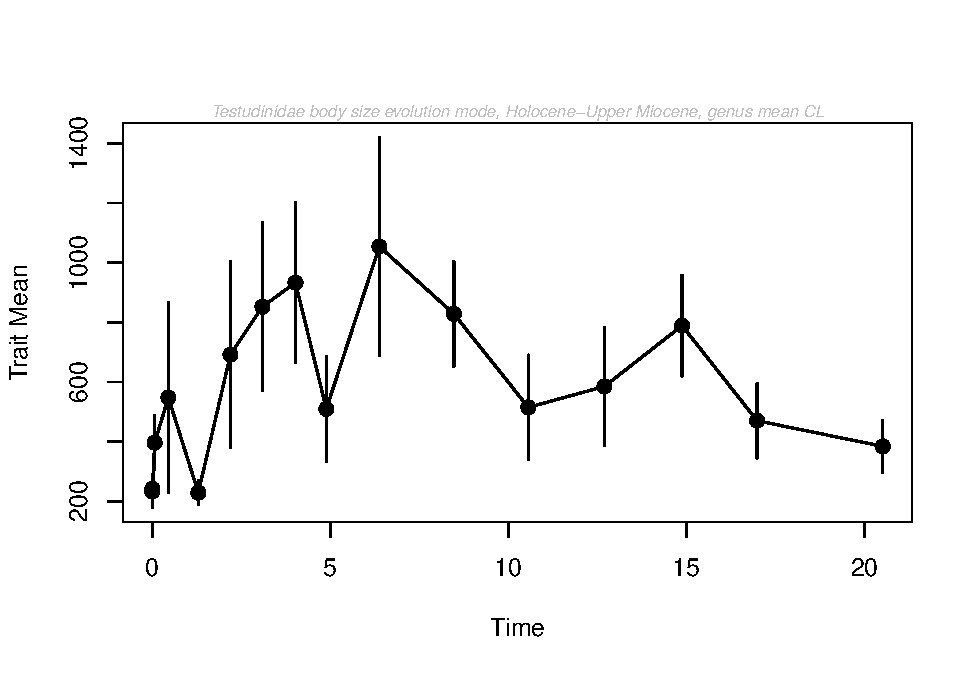
\includegraphics{MA_JJ_files/figure-latex/paleoTS plot with genus mean, excluding island species-1.pdf}
\caption{paleoTS plot with genus mean, excluding island species}
\end{figure}

\begin{longtable}[]{@{}lrrrr@{}}
\caption{Model-fitting results for testudinidae, genera, excluding
insular species}\tabularnewline
\toprule
& logL & K & AICc & Akaike.wt\tabularnewline
\midrule
\endfirsthead
\toprule
& logL & K & AICc & Akaike.wt\tabularnewline
\midrule
\endhead
GRW & -65.94462 & 2 & 137.6035 & 0.175\tabularnewline
URW & -66.03667 & 1 & 134.5733 & 0.796\tabularnewline
Stasis & -67.73195 & 2 & 141.1782 & 0.029\tabularnewline
\bottomrule
\end{longtable}

\newpage

\subsection{insular (excluding
continental)}\label{insular-excluding-continental}

\subsubsection{individuals (insular)}\label{individuals-insular}

\begin{figure}[htbp]
\centering
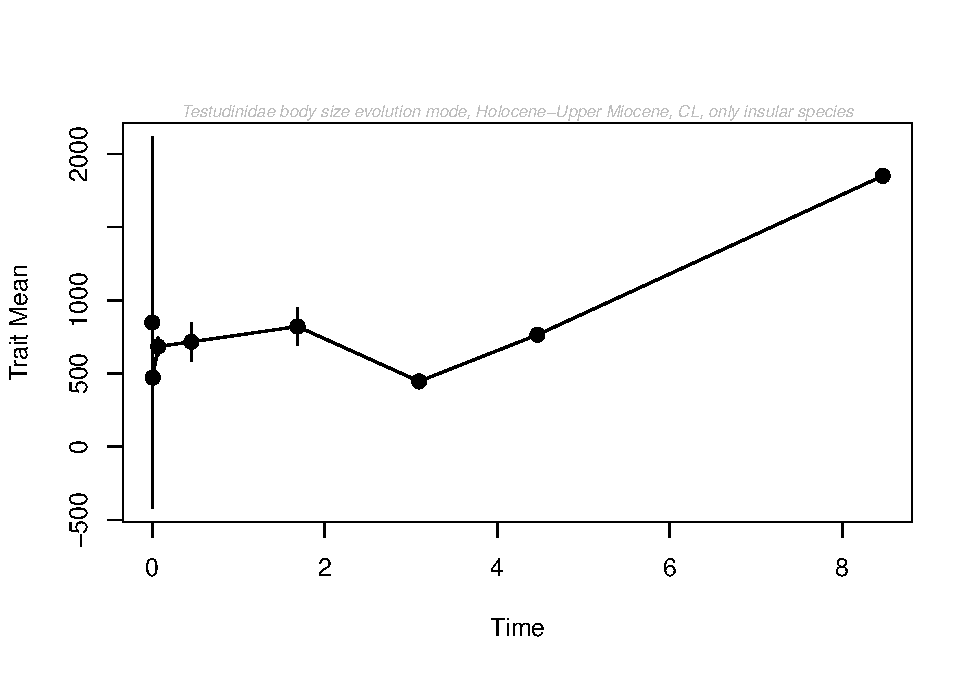
\includegraphics{MA_JJ_files/figure-latex/paleoTS, individuals, exluding continental species-1.pdf}
\caption{individuals, excluding continental species}
\end{figure}

\begin{longtable}[]{@{}lrrrr@{}}
\caption{Model-fitting results for testudinidae, individuals, only
insular species}\tabularnewline
\toprule
& logL & K & AICc & Akaike.wt\tabularnewline
\midrule
\endfirsthead
\toprule
& logL & K & AICc & Akaike.wt\tabularnewline
\midrule
\endhead
GRW & -62.23202 & 2 & 131.4640 & 0.000\tabularnewline
URW & -52.89195 & 1 & 108.5839 & 0.999\tabularnewline
Stasis & -58.14309 & 2 & 123.2862 & 0.001\tabularnewline
\bottomrule
\end{longtable}

\newpage

\subsubsection{species (insular)}\label{species-insular}

\begin{figure}[htbp]
\centering
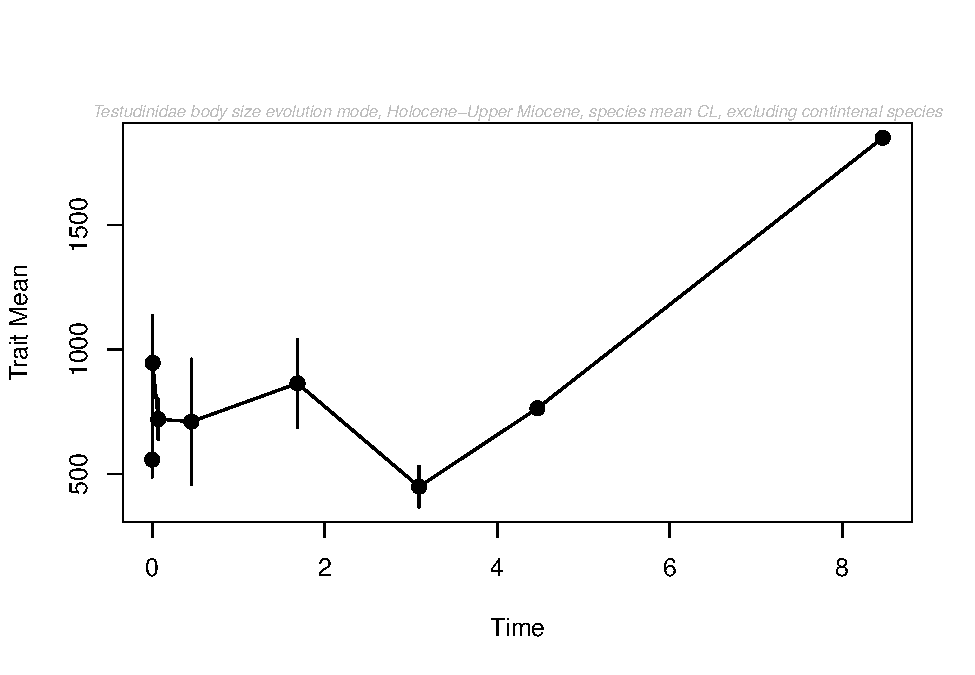
\includegraphics{MA_JJ_files/figure-latex/paleoTS plot with species mean, excluding continental species-1.pdf}
\caption{paleoTS plot with species mean, only insular species}
\end{figure}

\begin{longtable}[]{@{}lrrrr@{}}
\caption{Model-fitting results for testudinidae, species, only insular
species}\tabularnewline
\toprule
& logL & K & AICc & Akaike.wt\tabularnewline
\midrule
\endfirsthead
\toprule
& logL & K & AICc & Akaike.wt\tabularnewline
\midrule
\endhead
GRW & -60.91398 & 2 & 127.8280 & 0.020\tabularnewline
URW & -62.36871 & 1 & 127.3088 & 0.026\tabularnewline
Stasis & -57.04727 & 2 & 120.0945 & 0.954\tabularnewline
\bottomrule
\end{longtable}

\newpage

\subsubsection{genera (insular)}\label{genera-insular}

\begin{figure}[htbp]
\centering
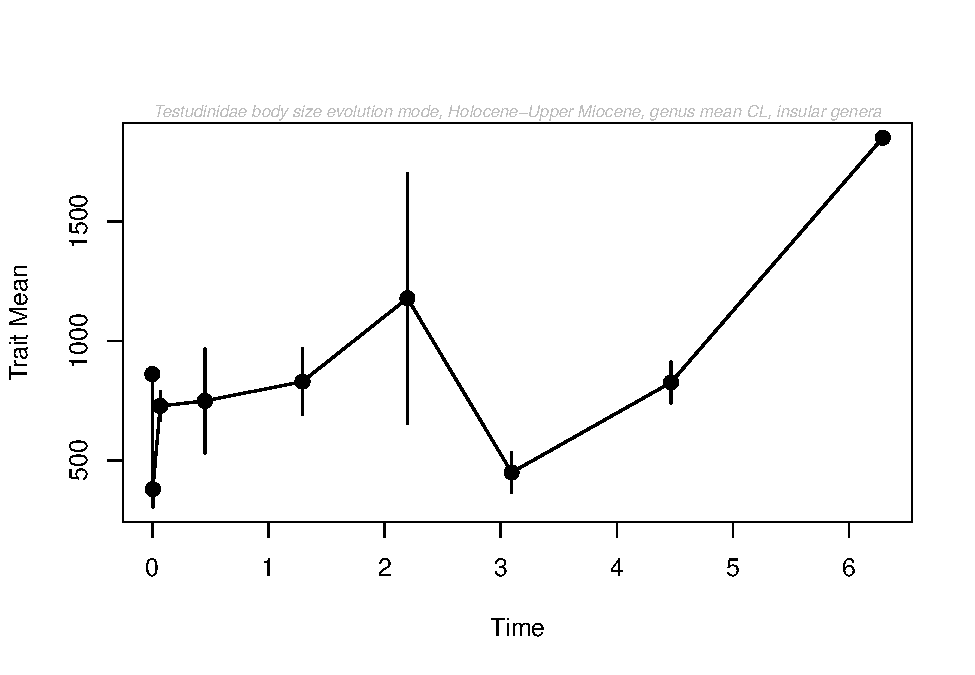
\includegraphics{MA_JJ_files/figure-latex/paleoTS plot with genus mean, excluding continental species-1.pdf}
\caption{paleoTS plot with genus mean, only insular species}
\end{figure}

\begin{longtable}[]{@{}lrrrr@{}}
\caption{Model-fitting results for testudinidae, genera, only insular
species}\tabularnewline
\toprule
& logL & K & AICc & Akaike.wt\tabularnewline
\midrule
\endfirsthead
\toprule
& logL & K & AICc & Akaike.wt\tabularnewline
\midrule
\endhead
GRW & -60.79557 & 2 & 128.5911 & 0\tabularnewline
URW & -67.79820 & 1 & 138.3964 & 0\tabularnewline
Stasis & -52.91882 & 2 & 112.8376 & 1\tabularnewline
\bottomrule
\end{longtable}

\newpage

\subsection{play with time bins: no bins (mean age of each sample ==
tt)}\label{play-with-time-bins-no-bins-mean-age-of-each-sample-tt}

\begin{figure}[htbp]
\centering
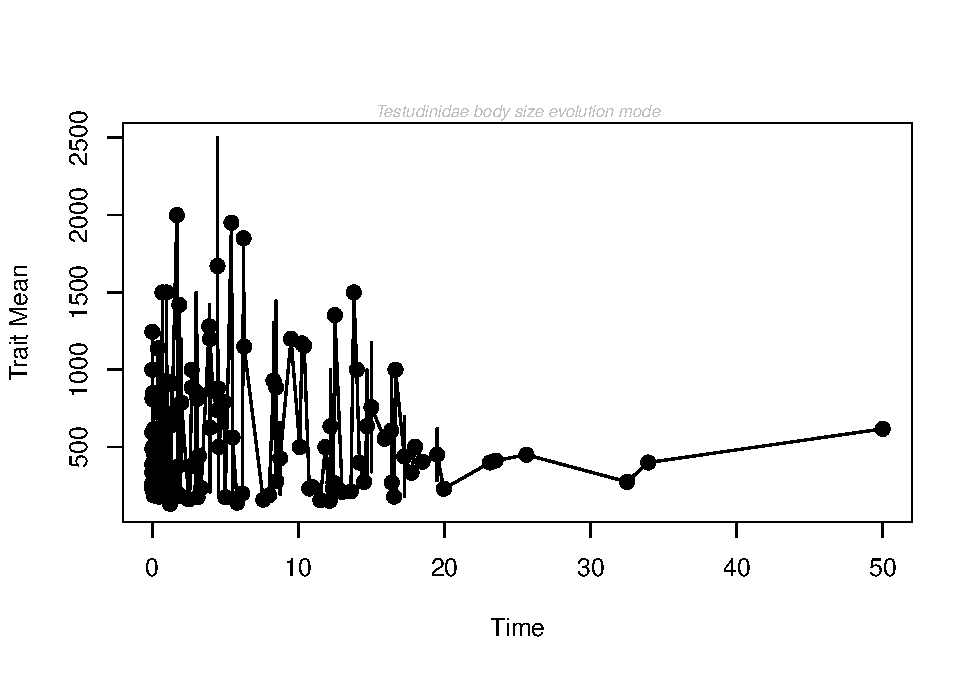
\includegraphics{MA_JJ_files/figure-latex/paleoTS with different time bins, no bins, genera-1.pdf}
\caption{Mean age of each sample as time bin, genera}
\end{figure}

\begin{longtable}[]{@{}lrrrr@{}}
\caption{Model-fitting results for testudinidae, no bins,
genera}\tabularnewline
\toprule
& logL & K & AICc & Akaike.wt\tabularnewline
\midrule
\endfirsthead
\toprule
& logL & K & AICc & Akaike.wt\tabularnewline
\midrule
\endhead
GRW & -963.1184 & 2 & 1930.347 & 0\tabularnewline
URW & -963.0117 & 1 & 1928.060 & 0\tabularnewline
Stasis & -841.6458 & 2 & 1687.402 & 1\tabularnewline
\bottomrule
\end{longtable}

\newpage

\subsection{Equal time bins}\label{equal-time-bins}

\subsubsection{individuals (equal bins)}\label{individuals-equal-bins}

\begin{longtable}[]{@{}rrrr@{}}
\caption{Time bins with age range, epoch name, mean age and
corresponding sample sizes (on individual, species and genus
level)}\tabularnewline
\toprule
tt & mm & vv & nn\tabularnewline
\midrule
\endfirsthead
\toprule
tt & mm & vv & nn\tabularnewline
\midrule
\endhead
0.00025 & 312.3935 & 59397.2190 & 240\tabularnewline
0.50025 & 443.0221 & 92434.1831 & 106\tabularnewline
1.50000 & 408.7154 & 166210.0663 & 65\tabularnewline
2.50000 & 511.5214 & 250980.0218 & 14\tabularnewline
3.50000 & 855.4545 & 491968.4502 & 22\tabularnewline
4.50000 & 856.8167 & 442457.0942 & 12\tabularnewline
5.50000 & 898.4286 & 665399.2857 & 7\tabularnewline
6.50000 & 1066.6667 & 685833.3333 & 3\tabularnewline
7.50000 & 169.3333 & 290.0833 & 3\tabularnewline
8.50000 & 439.0000 & 143244.5625 & 25\tabularnewline
9.50000 & 1200.0000 & 0.0000 & 1\tabularnewline
10.50000 & 633.0000 & 182138.8440 & 6\tabularnewline
11.50000 & 225.6000 & 24395.8000 & 5\tabularnewline
12.50000 & 297.8450 & 95170.7552 & 20\tabularnewline
13.50000 & 904.3333 & 420956.3333 & 3\tabularnewline
14.50000 & 662.1286 & 187942.8824 & 7\tabularnewline
15.50000 & 553.3333 & 192533.3333 & 3\tabularnewline
16.50000 & 532.6600 & 183446.2780 & 5\tabularnewline
17.50000 & 410.2308 & 80269.6923 & 13\tabularnewline
18.50000 & 405.0000 & 2450.0000 & 2\tabularnewline
19.50000 & 353.5000 & 32382.3333 & 4\tabularnewline
23.50000 & 406.2500 & 78.1250 & 2\tabularnewline
25.50000 & 450.0000 & 0.0000 & 1\tabularnewline
32.50000 & 275.0000 & 0.0000 & 1\tabularnewline
33.50000 & 400.0000 & 0.0000 & 1\tabularnewline
49.50000 & 617.5000 & 612.5000 & 2\tabularnewline
\bottomrule
\end{longtable}

\begin{figure}[htbp]
\centering
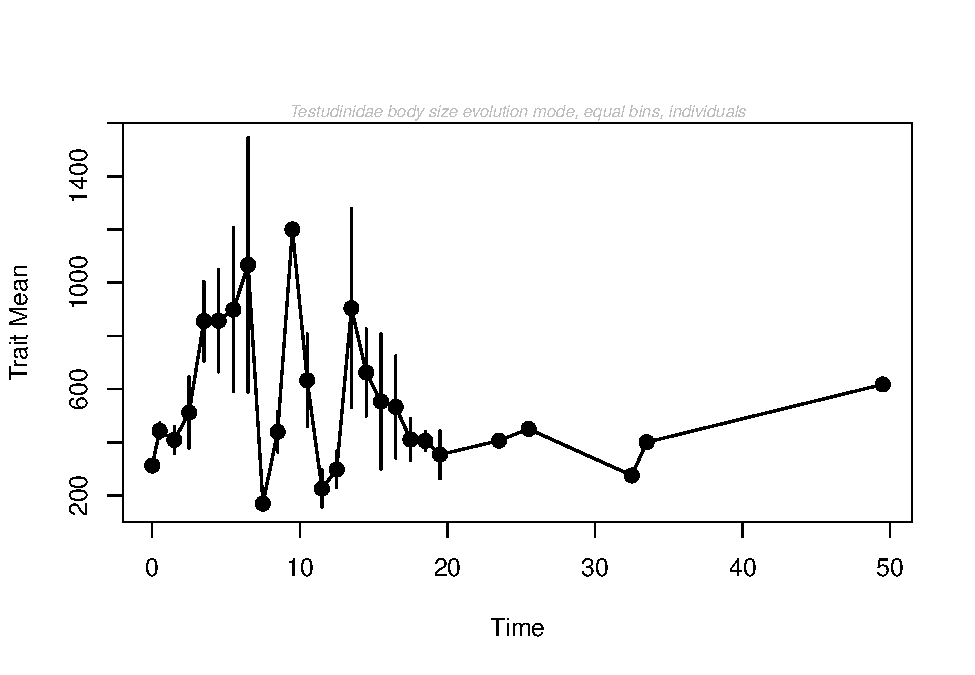
\includegraphics{MA_JJ_files/figure-latex/Play around with time bins, larger equal bins, individuals-1.pdf}
\caption{Equal bins, individuals}
\end{figure}

\begin{longtable}[]{@{}lrrrr@{}}
\caption{Model-fitting results for testudinidae, equal time bins,
individuals}\tabularnewline
\toprule
& logL & K & AICc & Akaike.wt\tabularnewline
\midrule
\endfirsthead
\toprule
& logL & K & AICc & Akaike.wt\tabularnewline
\midrule
\endhead
GRW & -181.0860 & 2 & 366.7174 & 0.001\tabularnewline
URW & -182.5837 & 1 & 367.3413 & 0.001\tabularnewline
Stasis & -174.2101 & 2 & 352.9656 & 0.998\tabularnewline
\bottomrule
\end{longtable}

\newpage

\subsubsection{species (equal bins)}\label{species-equal-bins}

\begin{longtable}[]{@{}rrrr@{}}
\caption{Time bins with age range, epoch name, mean age and
corresponding sample sizes (on individual, species and genus
level)}\tabularnewline
\toprule
tt & mm & vv & nn\tabularnewline
\midrule
\endfirsthead
\toprule
tt & mm & vv & nn\tabularnewline
\midrule
\endhead
0.00025 & 397.6667 & 96349.541 & 58\tabularnewline
0.50025 & 561.9257 & 113439.136 & 27\tabularnewline
1.50000 & 620.6031 & 318426.391 & 23\tabularnewline
2.50000 & 505.6300 & 220722.247 & 10\tabularnewline
3.50000 & 685.2500 & 336444.138 & 11\tabularnewline
4.50000 & 951.2000 & 525502.647 & 9\tabularnewline
5.50000 & 803.6250 & 719333.562 & 4\tabularnewline
6.50000 & 1066.6667 & 685833.333 & 3\tabularnewline
7.50000 & 174.2500 & 435.125 & 2\tabularnewline
8.50000 & 659.7000 & 290503.185 & 9\tabularnewline
9.50000 & 1200.0000 & 0.000 & 1\tabularnewline
10.50000 & 633.0000 & 182138.844 & 6\tabularnewline
11.50000 & 328.5000 & 58824.500 & 2\tabularnewline
12.50000 & 498.0192 & 226588.614 & 7\tabularnewline
13.50000 & 904.3333 & 420956.333 & 3\tabularnewline
14.50000 & 576.6500 & 161906.135 & 6\tabularnewline
15.50000 & 553.3333 & 0.000 & 1\tabularnewline
16.50000 & 532.6600 & 183446.278 & 5\tabularnewline
17.50000 & 428.2292 & 49344.877 & 4\tabularnewline
18.50000 & 405.0000 & 0.000 & 1\tabularnewline
19.50000 & 377.3333 & 44841.333 & 3\tabularnewline
23.50000 & 406.2500 & 0.000 & 1\tabularnewline
25.50000 & 450.0000 & 0.000 & 1\tabularnewline
32.50000 & 275.0000 & 0.000 & 1\tabularnewline
33.50000 & 400.0000 & 0.000 & 1\tabularnewline
49.50000 & 617.5000 & 0.000 & 1\tabularnewline
\bottomrule
\end{longtable}

\begin{figure}[htbp]
\centering
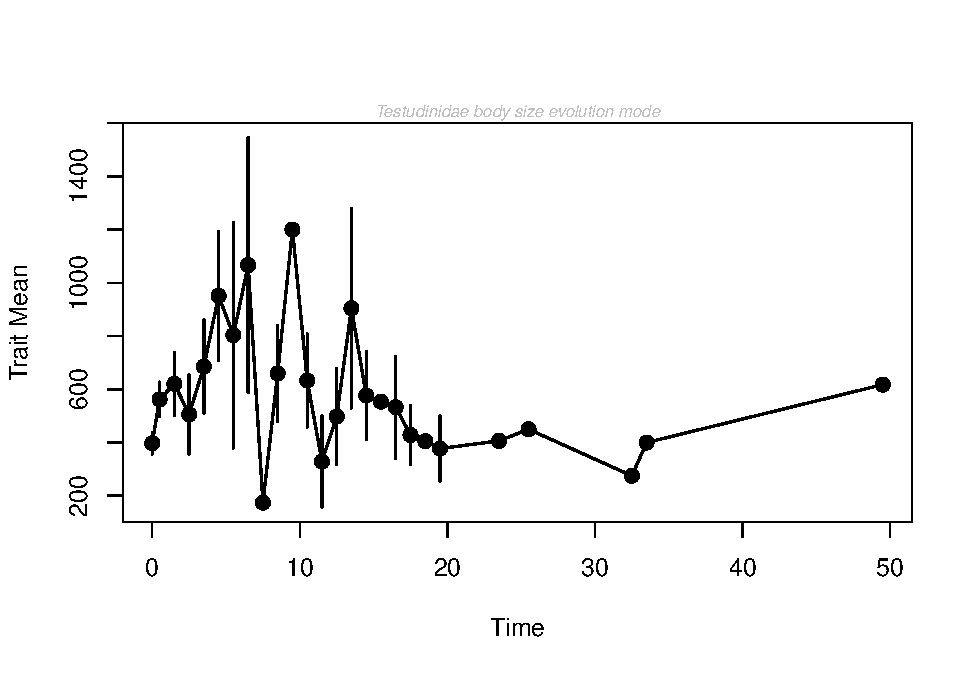
\includegraphics{MA_JJ_files/figure-latex/Play around with time bins, equal bin, species level-1.pdf}
\caption{Equal bins, species}
\end{figure}

\begin{longtable}[]{@{}lrrrr@{}}
\caption{Model-fitting results for testudinidae, equal time bins,
species}\tabularnewline
\toprule
& logL & K & AICc & Akaike.wt\tabularnewline
\midrule
\endfirsthead
\toprule
& logL & K & AICc & Akaike.wt\tabularnewline
\midrule
\endhead
GRW & -177.3909 & 2 & 359.3272 & 0.011\tabularnewline
URW & -178.7626 & 1 & 359.6991 & 0.010\tabularnewline
Stasis & -172.9454 & 2 & 350.4363 & 0.979\tabularnewline
\bottomrule
\end{longtable}

\newpage

\subsubsection{genera (equal bins)}\label{genera-equal-bins}

\begin{longtable}[]{@{}rrrr@{}}
\caption{Time bins with age range, epoch name, mean age and
corresponding sample sizes (on individual, species and genus
level)}\tabularnewline
\toprule
tt & mm & vv & nn\tabularnewline
\midrule
\endfirsthead
\toprule
tt & mm & vv & nn\tabularnewline
\midrule
\endhead
0.00025 & 335.6380 & 49292.698 & 17\tabularnewline
0.50025 & 547.6849 & 98246.139 & 12\tabularnewline
1.50000 & 558.2001 & 194613.806 & 11\tabularnewline
2.50000 & 627.7867 & 235547.641 & 5\tabularnewline
3.50000 & 758.8929 & 285072.539 & 7\tabularnewline
4.50000 & 961.8833 & 621030.522 & 6\tabularnewline
5.50000 & 1020.0000 & 797671.000 & 3\tabularnewline
6.50000 & 850.0000 & 845000.000 & 2\tabularnewline
7.50000 & 174.2500 & 435.125 & 2\tabularnewline
8.50000 & 770.9667 & 229304.487 & 6\tabularnewline
9.50000 & 1200.0000 & 0.000 & 1\tabularnewline
10.50000 & 527.1000 & 143534.355 & 5\tabularnewline
11.50000 & 328.5000 & 58824.500 & 2\tabularnewline
12.50000 & 602.1210 & 291476.249 & 5\tabularnewline
13.50000 & 904.3333 & 420956.333 & 3\tabularnewline
14.50000 & 624.4800 & 183271.727 & 5\tabularnewline
15.50000 & 553.3333 & 0.000 & 1\tabularnewline
16.50000 & 532.6600 & 183446.278 & 5\tabularnewline
17.50000 & 366.5238 & 41915.395 & 3\tabularnewline
18.50000 & 405.0000 & 0.000 & 1\tabularnewline
19.50000 & 377.3333 & 44841.333 & 3\tabularnewline
23.50000 & 406.2500 & 0.000 & 1\tabularnewline
25.50000 & 450.0000 & 0.000 & 1\tabularnewline
32.50000 & 275.0000 & 0.000 & 1\tabularnewline
33.50000 & 400.0000 & 0.000 & 1\tabularnewline
49.50000 & 617.5000 & 0.000 & 1\tabularnewline
\bottomrule
\end{longtable}

\begin{figure}[htbp]
\centering
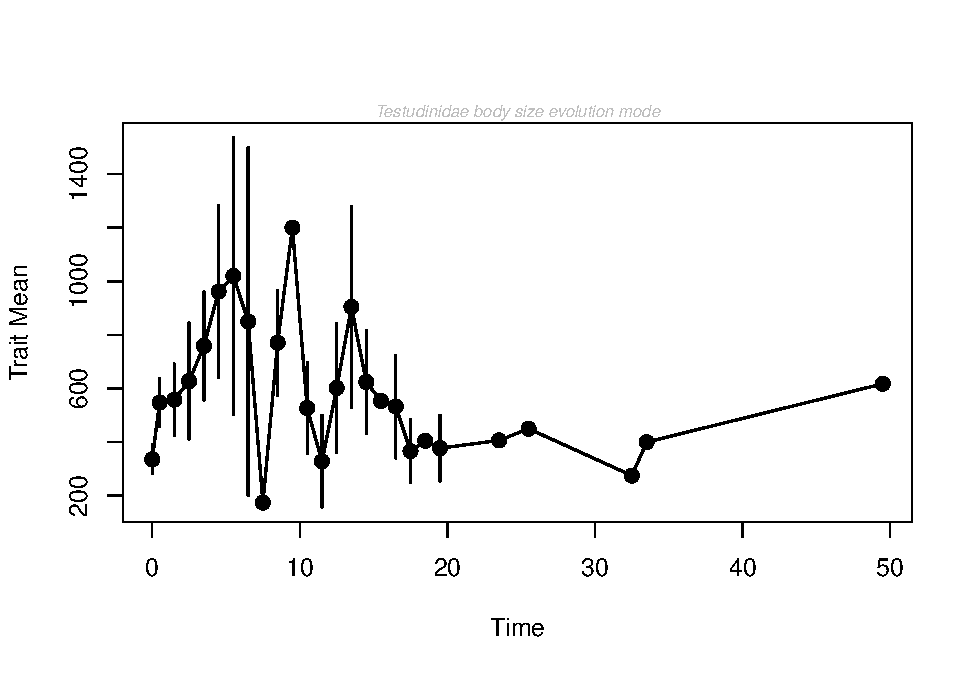
\includegraphics{MA_JJ_files/figure-latex/Play around with time bins, generic level-1.pdf}
\caption{Equal bins, genera}
\end{figure}

\begin{longtable}[]{@{}lrrrr@{}}
\caption{Model-fitting results for testudinidae, equal time bins,
genera}\tabularnewline
\toprule
& logL & K & AICc & Akaike.wt\tabularnewline
\midrule
\endfirsthead
\toprule
& logL & K & AICc & Akaike.wt\tabularnewline
\midrule
\endhead
GRW & -179.4504 & 2 & 363.4462 & 0.008\tabularnewline
URW & -178.8180 & 1 & 359.8099 & 0.051\tabularnewline
Stasis & -174.7233 & 2 & 353.9921 & 0.940\tabularnewline
\bottomrule
\end{longtable}

\subsection{larger equal bins}\label{larger-equal-bins}

\subsubsection{genera (larger equal
bins)}\label{genera-larger-equal-bins}

\begin{longtable}[]{@{}rrrr@{}}
\caption{Time bins with age range, epoch name, mean age and
corresponding sample sizes (on individual, species and genus
level)}\tabularnewline
\toprule
tt & mm & vv & nn\tabularnewline
\midrule
\endfirsthead
\toprule
tt & mm & vv & nn\tabularnewline
\midrule
\endhead
0.5 & 404.7783 & 74680.998 & 21\tabularnewline
1.5 & 558.2001 & 194613.806 & 11\tabularnewline
2.5 & 627.7867 & 235547.641 & 5\tabularnewline
3.5 & 758.8929 & 285072.539 & 7\tabularnewline
4.5 & 961.8833 & 621030.522 & 6\tabularnewline
5.5 & 1020.0000 & 797671.000 & 3\tabularnewline
6.5 & 850.0000 & 845000.000 & 2\tabularnewline
7.5 & 174.2500 & 435.125 & 2\tabularnewline
8.5 & 770.9667 & 229304.487 & 6\tabularnewline
9.5 & 1200.0000 & 0.000 & 1\tabularnewline
10.5 & 527.1000 & 143534.355 & 5\tabularnewline
11.5 & 328.5000 & 58824.500 & 2\tabularnewline
12.5 & 602.1210 & 291476.249 & 5\tabularnewline
13.5 & 904.3333 & 420956.333 & 3\tabularnewline
14.5 & 624.4800 & 183271.727 & 5\tabularnewline
15.5 & 553.3333 & 0.000 & 1\tabularnewline
16.5 & 532.6600 & 183446.278 & 5\tabularnewline
17.5 & 366.5238 & 41915.395 & 3\tabularnewline
18.5 & 405.0000 & 0.000 & 1\tabularnewline
19.5 & 377.3333 & 44841.333 & 3\tabularnewline
23.5 & 406.2500 & 0.000 & 1\tabularnewline
25.5 & 450.0000 & 0.000 & 1\tabularnewline
32.5 & 275.0000 & 0.000 & 1\tabularnewline
33.5 & 400.0000 & 0.000 & 1\tabularnewline
49.5 & 617.5000 & 0.000 & 1\tabularnewline
\bottomrule
\end{longtable}

\begin{figure}[htbp]
\centering
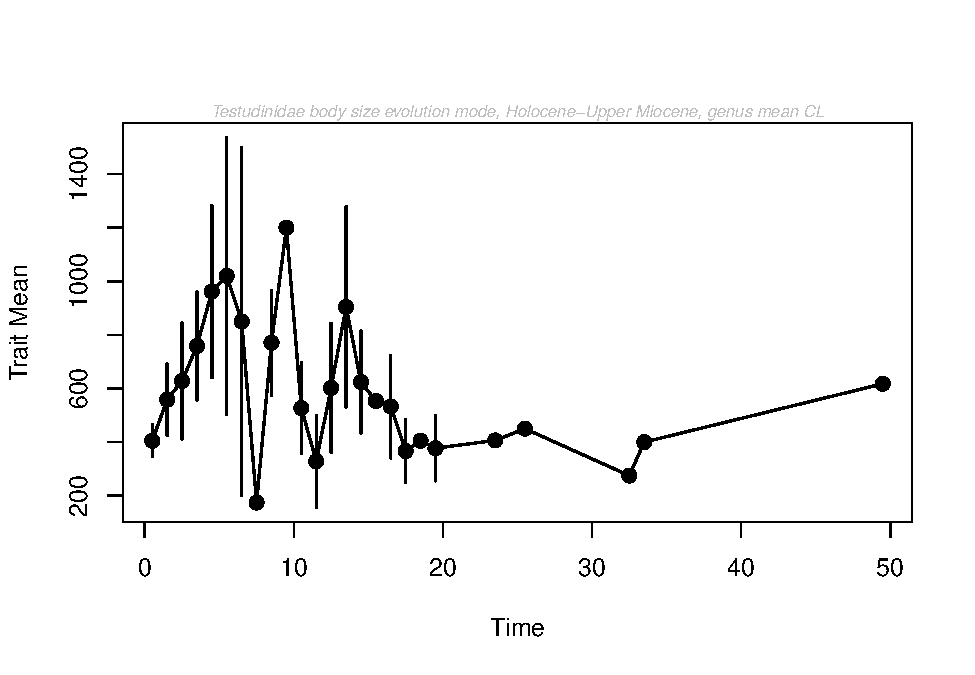
\includegraphics{MA_JJ_files/figure-latex/Play around with larger time bins, generic level-1.pdf}
\caption{Larger equal bins, genera}
\end{figure}

\begin{longtable}[]{@{}lrrrr@{}}
\caption{Model-fitting results for testudinidae, larger equal time bins,
genera}\tabularnewline
\toprule
& logL & K & AICc & Akaike.wt\tabularnewline
\midrule
\endfirsthead
\toprule
& logL & K & AICc & Akaike.wt\tabularnewline
\midrule
\endhead
GRW & -172.6279 & 2 & 349.8272 & 0.036\tabularnewline
URW & -172.9972 & 1 & 348.1763 & 0.082\tabularnewline
Stasis & -169.4260 & 2 & 343.4234 & 0.882\tabularnewline
\bottomrule
\end{longtable}

\newpage

\subsection{per continent}\label{per-continent}

\subsubsection{Africa, individuals}\label{africa-individuals}

\begin{longtable}[]{@{}rrrr@{}}
\caption{paleoTS object (mm= mean CL, nn = sample size, vv = variance
(CL), tt = Age)}\tabularnewline
\toprule
mm & nn & vv & tt\tabularnewline
\midrule
\endfirsthead
\toprule
mm & nn & vv & tt\tabularnewline
\midrule
\endhead
848.6396 & 111 & 176705032.40 & 0.0000005\tabularnewline
315.7257 & 113 & 84989.64 & 0.0058500\tabularnewline
132.0000 & 1 & 0.00 & 0.4535000\tabularnewline
192.3000 & 6 & 11633.02 & 1.6845000\tabularnewline
1000.0000 & 1 & 0.00 & 3.0940000\tabularnewline
0.0000 & 4 & 0.00 & 4.4660000\tabularnewline
1446.0000 & 1 & 0.00 & 8.4700000\tabularnewline
412.2000 & 15 & 73921.74 & 19.5000000\tabularnewline
\bottomrule
\end{longtable}

\begin{figure}[htbp]
\centering
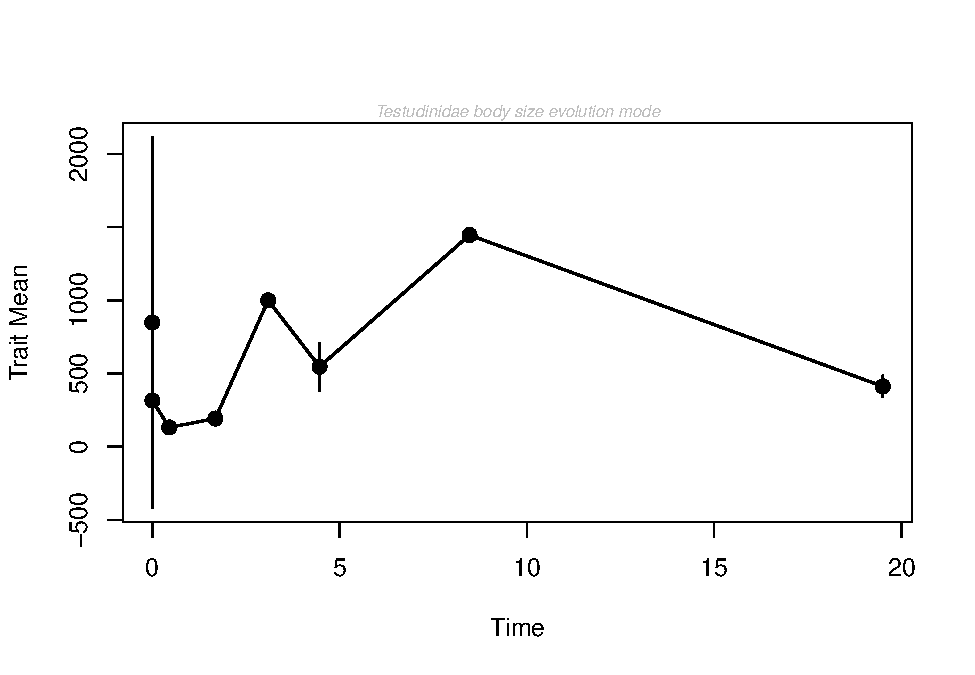
\includegraphics{MA_JJ_files/figure-latex/paleoTS, individuals, Africa-1.pdf}
\caption{Africa, individuals}
\end{figure}

\begin{longtable}[]{@{}lrrrr@{}}
\caption{Model-fitting results for testudinidae, individuals,
Africa}\tabularnewline
\toprule
& logL & K & AICc & Akaike.wt\tabularnewline
\midrule
\endfirsthead
\toprule
& logL & K & AICc & Akaike.wt\tabularnewline
\midrule
\endhead
GRW & -69.73883 & 2 & 146.4777 & 0.00\tabularnewline
URW & -62.56518 & 1 & 127.9304 & 0.99\tabularnewline
Stasis & -65.08256 & 2 & 137.1651 & 0.01\tabularnewline
\bottomrule
\end{longtable}

\newpage

\subsubsection{Europe, individuals}\label{europe-individuals}

\begin{longtable}[]{@{}rrrr@{}}
\caption{paleoTS object (mm= mean CL, nn = sample size, vv = variance
(CL), tt = Age)}\tabularnewline
\toprule
mm & nn & vv & tt\tabularnewline
\midrule
\endfirsthead
\toprule
mm & nn & vv & tt\tabularnewline
\midrule
\endhead
187.3771 & 35 & 3707.446 & 0.00585\tabularnewline
616.6667 & 3 & 138802.333 & 0.06885\tabularnewline
377.8167 & 12 & 75333.898 & 0.45350\tabularnewline
731.5786 & 14 & 306198.902 & 1.68450\tabularnewline
0.0000 & 6 & 0.000 & 3.09400\tabularnewline
1283.1429 & 14 & 566267.670 & 4.46600\tabularnewline
0.0000 & 35 & 0.000 & 8.47000\tabularnewline
0.0000 & 30 & 0.000 & 13.78900\tabularnewline
482.2167 & 6 & 162024.202 & 19.50000\tabularnewline
489.5000 & 5 & 13832.500 & 36.51500\tabularnewline
\bottomrule
\end{longtable}

\begin{figure}[htbp]
\centering
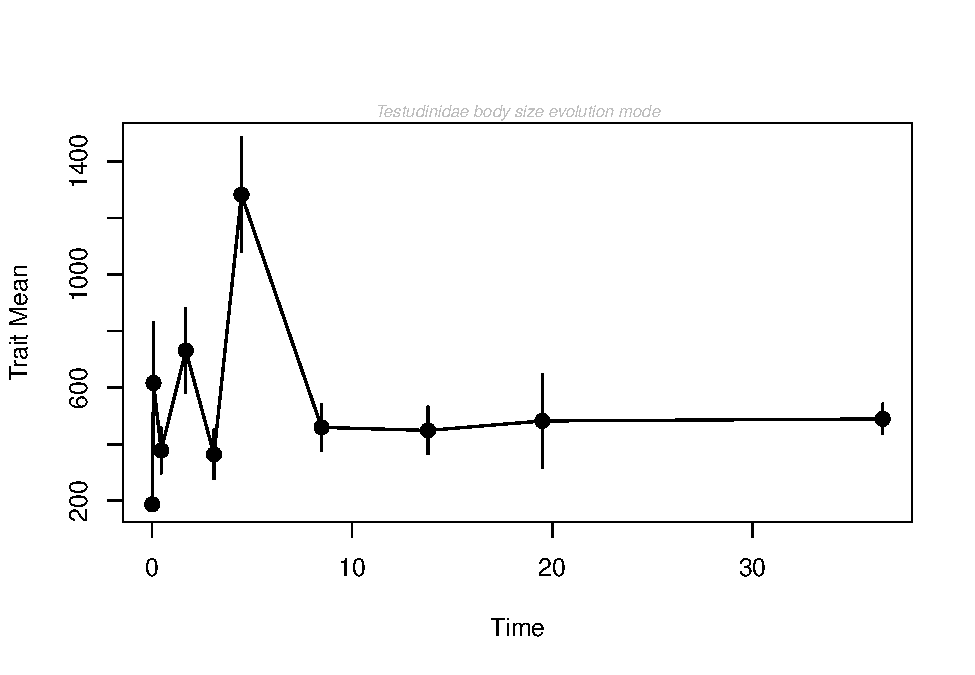
\includegraphics{MA_JJ_files/figure-latex/paleoTS, individuals, Europe-1.pdf}
\caption{Europe, individuals}
\end{figure}

\begin{longtable}[]{@{}lrrrr@{}}
\caption{Model-fitting results for testudinidae, individuals,
Europe}\tabularnewline
\toprule
& logL & K & AICc & Akaike.wt\tabularnewline
\midrule
\endfirsthead
\toprule
& logL & K & AICc & Akaike.wt\tabularnewline
\midrule
\endhead
GRW & -73.23814 & 2 & 152.4763 & 0.001\tabularnewline
URW & -74.54846 & 1 & 151.6683 & 0.002\tabularnewline
Stasis & -66.43459 & 2 & 138.8692 & 0.997\tabularnewline
\bottomrule
\end{longtable}

\newpage

\subsubsection{America, individuals}\label{america-individuals}

\begin{longtable}[]{@{}rrrr@{}}
\caption{paleoTS object (mm= mean CL, nn = sample size, vv = variance
(CL), tt = Age)}\tabularnewline
\toprule
mm & nn & vv & tt\tabularnewline
\midrule
\endfirsthead
\toprule
mm & nn & vv & tt\tabularnewline
\midrule
\endhead
254.5369 & 807 & 389794806.8 & 0.0000005\tabularnewline
0.0000 & 69 & 0.0 & 0.0058500\tabularnewline
0.0000 & 43 & 0.0 & 0.0688500\tabularnewline
0.0000 & 35 & 0.0 & 0.4535000\tabularnewline
0.0000 & 49 & 0.0 & 1.6845000\tabularnewline
0.0000 & 12 & 0.0 & 3.0940000\tabularnewline
0.0000 & 9 & 0.0 & 4.4660000\tabularnewline
467.4214 & 14 & 117249.1 & 8.4700000\tabularnewline
0.0000 & 8 & 0.0 & 13.7890000\tabularnewline
0.0000 & 4 & 0.0 & 19.5000000\tabularnewline
450.0000 & 1 & 0.0 & 36.5150000\tabularnewline
\bottomrule
\end{longtable}

\begin{figure}[htbp]
\centering
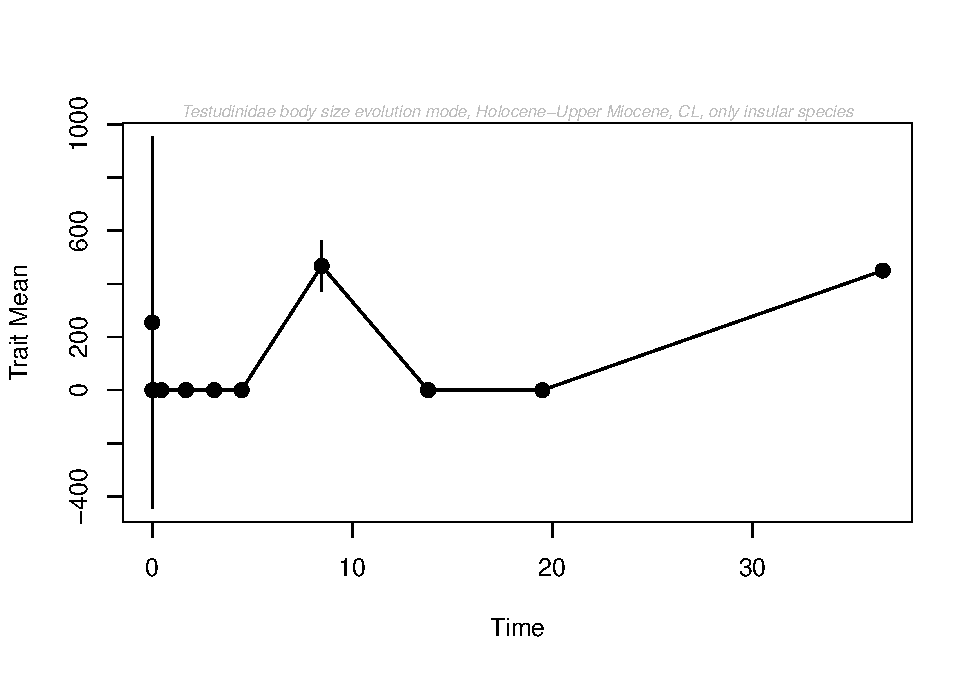
\includegraphics{MA_JJ_files/figure-latex/paleoTS, individuals, America-1.pdf}
\caption{America, individuals}
\end{figure}

\begin{longtable}[]{@{}lrrrr@{}}
\caption{Model-fitting results for testudinidae, individuals,
America}\tabularnewline
\toprule
& logL & K & AICc & Akaike.wt\tabularnewline
\midrule
\endfirsthead
\toprule
& logL & K & AICc & Akaike.wt\tabularnewline
\midrule
\endhead
GRW & -64.72009 & 2 & 135.1545 & 0.130\tabularnewline
URW & -64.43046 & 1 & 131.3609 & 0.864\tabularnewline
Stasis & -67.81075 & 2 & 141.3358 & 0.006\tabularnewline
\bottomrule
\end{longtable}

\newpage

\subsubsection{Asia, individuals}\label{asia-individuals}

\begin{longtable}[]{@{}rrrr@{}}
\caption{paleoTS object (mm= mean CL, nn = sample size, vv = variance
(CL), tt = Age)}\tabularnewline
\toprule
mm & nn & vv & tt\tabularnewline
\midrule
\endfirsthead
\toprule
mm & nn & vv & tt\tabularnewline
\midrule
\endhead
137.2637 & 810 & 3.088779e+09 & 0.0000005\tabularnewline
279.0800 & 35 & 1.026795e+04 & 0.0058500\tabularnewline
270.0000 & 1 & 0.000000e+00 & 0.0688500\tabularnewline
989.5000 & 4 & 5.907610e+05 & 1.6845000\tabularnewline
1550.0000 & 4 & 3.333333e+03 & 3.0940000\tabularnewline
209.0000 & 2 & 2.420000e+02 & 4.4660000\tabularnewline
1950.0000 & 2 & 4.500000e+04 & 8.4700000\tabularnewline
275.0000 & 1 & 0.000000e+00 & 36.5150000\tabularnewline
\bottomrule
\end{longtable}

\begin{figure}[htbp]
\centering
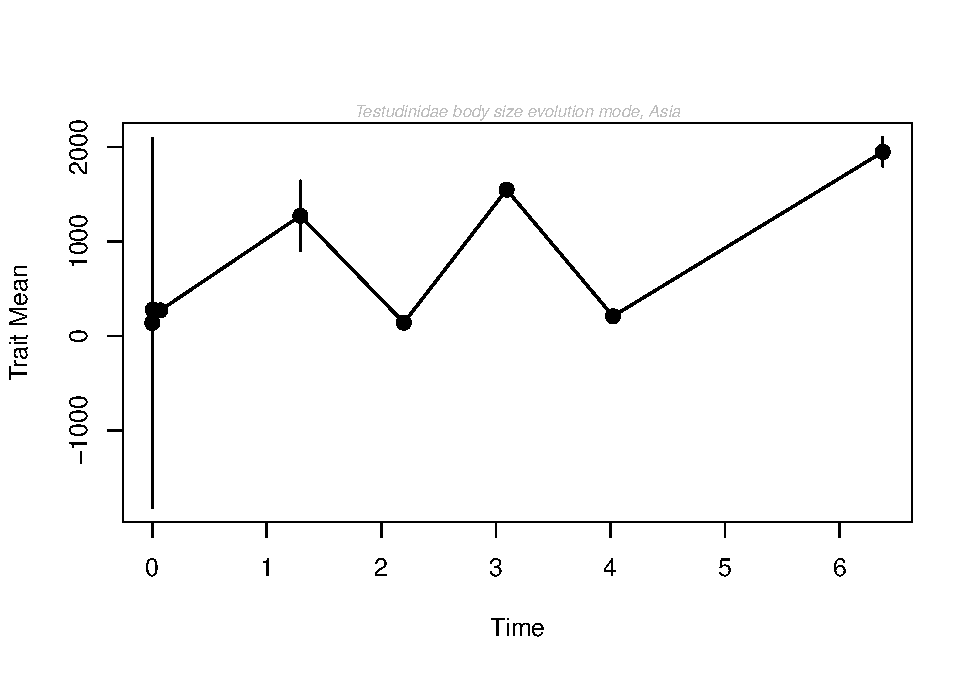
\includegraphics{MA_JJ_files/figure-latex/paleoTS, individuals, Asia-1.pdf}
\caption{individuals, Asia}
\end{figure}

\begin{longtable}[]{@{}lrrrr@{}}
\caption{Model-fitting results for testudinidae, individuals,
Asia}\tabularnewline
\toprule
& logL & K & AICc & Akaike.wt\tabularnewline
\midrule
\endfirsthead
\toprule
& logL & K & AICc & Akaike.wt\tabularnewline
\midrule
\endhead
GRW & -80.46824 & 2 & 167.9365 & 0\tabularnewline
URW & -58.38546 & 1 & 119.5709 & 1\tabularnewline
Stasis & -66.94216 & 2 & 140.8843 & 0\tabularnewline
\bottomrule
\end{longtable}

\newpage

\subsubsection{Eurasia, individuals}\label{eurasia-individuals}

\begin{longtable}[]{@{}rrrr@{}}
\caption{paleoTS object (mm= mean CL, nn = sample size, vv = variance
(CL), tt = Age)}\tabularnewline
\toprule
mm & nn & vv & tt\tabularnewline
\midrule
\endfirsthead
\toprule
mm & nn & vv & tt\tabularnewline
\midrule
\endhead
137.2637 & 810 & 3.088779e+09 & 0.0000005\tabularnewline
233.2286 & 70 & 9.019250e+03 & 0.0058500\tabularnewline
530.0000 & 4 & 1.225793e+05 & 0.0688500\tabularnewline
377.8167 & 12 & 7.533390e+04 & 0.4535000\tabularnewline
788.8944 & 18 & 3.505783e+05 & 1.6845000\tabularnewline
891.1111 & 9 & 4.104549e+05 & 3.0940000\tabularnewline
1148.8750 & 16 & 6.253894e+05 & 4.4660000\tabularnewline
547.2971 & 34 & 3.263311e+05 & 8.4700000\tabularnewline
448.7464 & 28 & 1.911266e+05 & 13.7890000\tabularnewline
482.2167 & 6 & 1.620242e+05 & 19.5000000\tabularnewline
453.7500 & 6 & 1.873438e+04 & 36.5150000\tabularnewline
\bottomrule
\end{longtable}

\begin{figure}[htbp]
\centering
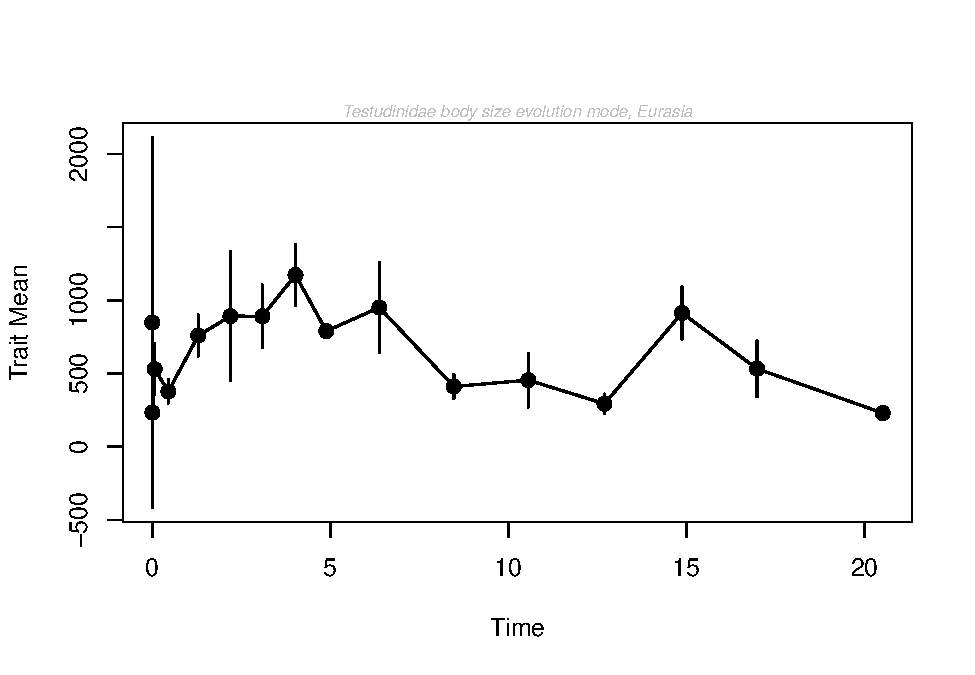
\includegraphics{MA_JJ_files/figure-latex/paleoTS, individuals, Eurasia-1.pdf}
\caption{individuals, Eurasia}
\end{figure}

\begin{longtable}[]{@{}lrrrr@{}}
\caption{Model-fitting results for testudinidae, individuals,
Asia}\tabularnewline
\toprule
& logL & K & AICc & Akaike.wt\tabularnewline
\midrule
\endfirsthead
\toprule
& logL & K & AICc & Akaike.wt\tabularnewline
\midrule
\endhead
GRW & -73.47268 & 2 & 152.6596 & 0.101\tabularnewline
URW & -73.64757 & 1 & 149.7951 & 0.425\tabularnewline
Stasis & -71.93258 & 2 & 149.5794 & 0.473\tabularnewline
\bottomrule
\end{longtable}


\end{document}
